%----------------------------------------------------------------------------------------
%	CHAPTER - LITERATURE REVIEW
%----------------------------------------------------------------------------------------

\chapter{Literature Review}

\label{ChapterLiteratureReview}

In the literature review chapter, an overview of existing research found in literature, that is relevant to the thesis statement of this paper, is given. Every \gls{srq} is discussed in its own sub-chapter where its relevance to the \gls{mrq} is elaborated. Each sub-chapter ends with a short conclusion and answers to the corresponding research question are given.
Figure \ref{fig:litreviewoverview} shows the correlation between the sub-chapters and the research questions. In chapter \ref{SectionLiteratureReviewSRQ1}, the different methods for user input in virtual reality are analysed The next chapter \ref{SectionLiteratureReviewSRQ2} focuses on existing data interaction patterns in virtual reality. By looking at strategies for the visualisation and manipulation of data, the third \gls{srq} is covered in chapter \ref{SectionLiteratureReviewSRQ3}. To wrap everything up, a conclusion of the literature review is presented in chapter \ref{SectionLiteratureReviewConclusion} which builds the base for the research design in chapter \ref{Research Method}.
\newline
\begin{figure}[h]
	\begin{center}
		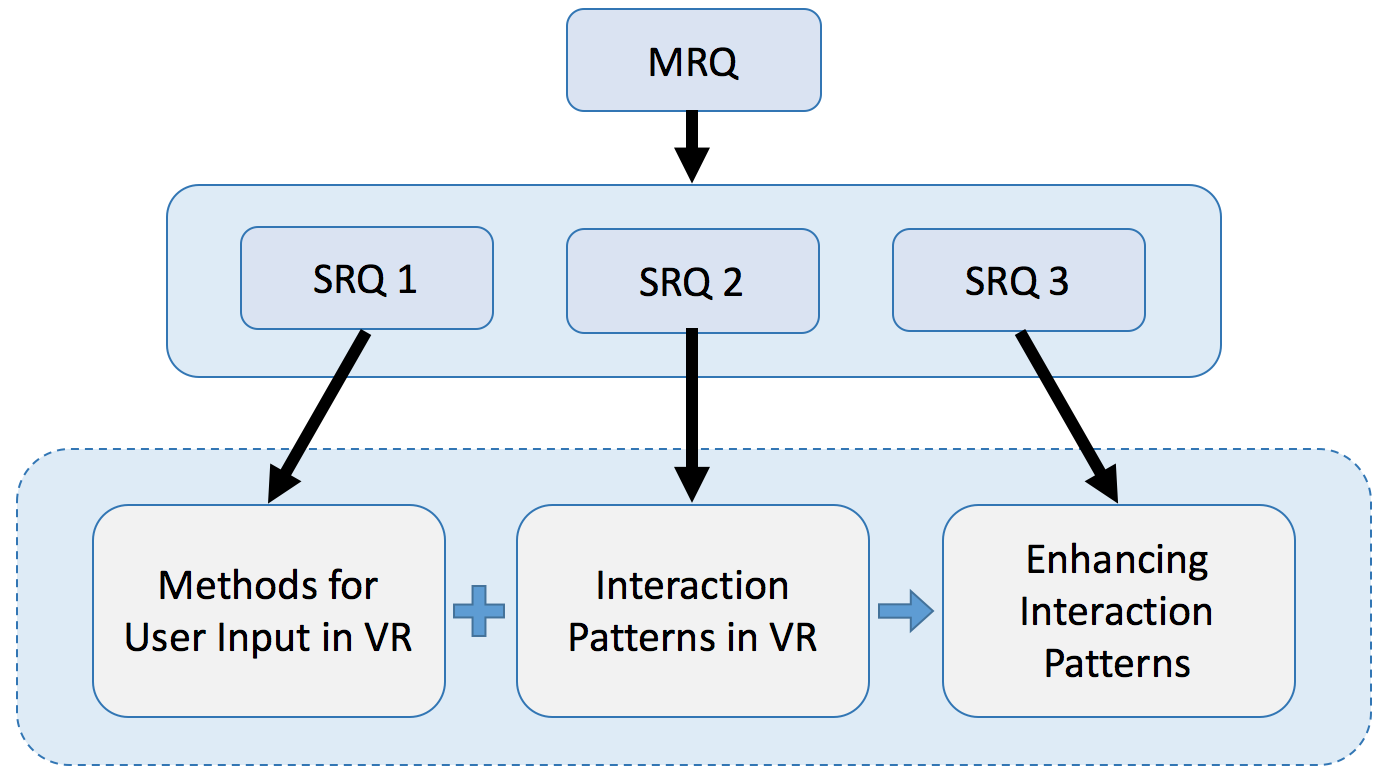
\includegraphics[width=12cm]{03_Figures/05_LitReview/LitReview_SRQ.png}
		\caption{Chapter 2 Overview}
		\label{fig:litreviewoverview}
	\end{center}
\end{figure}


%----------------------------------------------------------------------------------------
%	SECTION 1
%----------------------------------------------------------------------------------------

\section{Different Methods for User Input in Virtual Reality}

\label{SectionLiteratureReviewSRQ1}

This chapter deals with the first \gls{srq}, focusing on the currently used and researched different methods for user input in virtual reality. It starts with an introduction and an overview of the different methods while the subsequent chapters give more details on the individual methods.
\begin{framed}
	\textit{\gls{srq} 1: \srqonetext}
\end{framed}

%-----------------------------------
%	SUBSECTION 1
%-----------------------------------
\subsection{Introduction}

\gls{hci} itself has been worked and research on approximately from the 1950s onwards, where the main focus was on the direct manipulation of graphical objects with the mouse as well as gesture recognition \citep{Myers1998}. During this time however, gesture recognition was rather understood as devices that work with pen-based input devices and thus can recognize patterns that are drawn with these pens \citep{Myers1998}. In the regular interaction between human and machines these methods for user input are still fairly sufficient as even today we are completely relying on having a mouse/track-pad/touch-screen and a keyboard to interact with our devices. \newline
Virtual reality changes this quite a bit since wearing a \gls{hmd} with its own display obstructs the view on the so far used physical input devices. New solutions had to be found for this changed situation. An overview on the researched interaction patterns with virtual reality is shown in the following sub-chapter.


%-----------------------------------
%	SUBSECTION 2
%-----------------------------------

\subsection{Overview of the Different Methods}

The reviewed literature brought up different means in research to interact with the virtual reality environment. In order to review them in a more structured way, they have been grouped by their core technology (i.e. hand gestures, speech recognition etc.) on which they base on. Every core technology is discussed individually, its advantages and disadvantages are discussed, as well as their similarities or differences are explained.


\subsubsection{Hand Gestures}

\label{SubSubSectionHandGestures}

The by far most utilized and researched interaction method is hand gestures. Since we also heavily rely on this interaction pattern in real life with other human beings, it is fair to assume that the familiarity of it helps the research in a significant way whereas methods that rely on physical hardware often feel more distant. \newline
\cite{Pfeiffer2008} conducted an empirical study about conversational pointing gestures in virtual reality interaction where the focus lied on the system to recognize on which object the user was pointing at. \cite{Pfeiffer2008} distinguished between \gls{ifp} where the direction of where the index finger is pointing at, and \gls{gfp} where an imaginary line between the viewers eye and the tip of the index finger is drawn. Provided the objects are nod too close to each other (ca. 20cm), both methods had equal accuracy and success while tracked with two cameras from different angles and motion capturing \citep{Pfeiffer2008}. Figure \ref{fig:pointinggesture} shows the application of this in an identification game which was part of the empirical study.
\begin{figure}[h]
	\begin{center}
		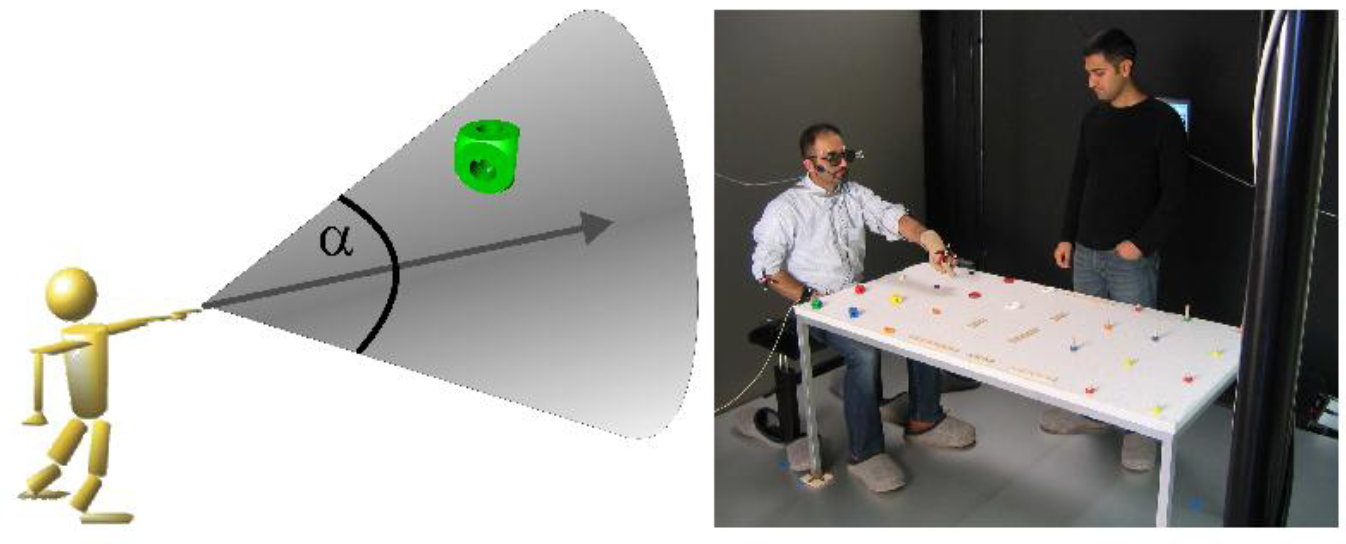
\includegraphics[width=10cm]{03_Figures/05_LitReview/Pfeiffer2008_Pointing.png}
		\caption[Cone-based model for extension of pointing gestures refined for identification game]{Cone-based model for extension of pointing gestures (left) refined for identification game (right) \citep{Pfeiffer2008}}
		\label{fig:pointinggesture}
	\end{center}
\end{figure}
\newline
A similar approach has been research by \cite{Rautaray2011} who used a single camera with an application that did the image capturing, locating the hand and its orientation and finally modelling the gesture to find a match for predefined gestures. The focus relied on simple gestures for \textit{punch} (three fingers), \textit{grab} (fist), \textit{throw} (five fingers), and to \textit{move forward} (thumb up) within a simple \gls{vr} game \citep{Rautaray2011}. The recognition rate was between 80\% and 94\% (depending on the gesture), which might not be accurate enough for practical use cases as also acknowledged by \cite{Rautaray2011}. \newline
In a more recent study of \cite{Khundam2015}, it was not cameras that were used to track the hand gestures but a Leap Motion (an in-air controller) attached to the front of an Oculus Rift. Figure \ref{fig:leapmotion} shows the different gestures that were implemented by \cite{Khundam2015} in order to navigate within a \gls{ve}. Depending on how far the hand is moved towards a certain angle, the speed of the movement can be influenced to increase or decrease it \citep{Khundam2015}. Although the applied gestures are understandable and easy to learn, they still bring some unfamiliarity with them since in real life movement already has a specific gesture which however utilizes the legs and not the hands.
\begin{figure}[h]
	\begin{center}
		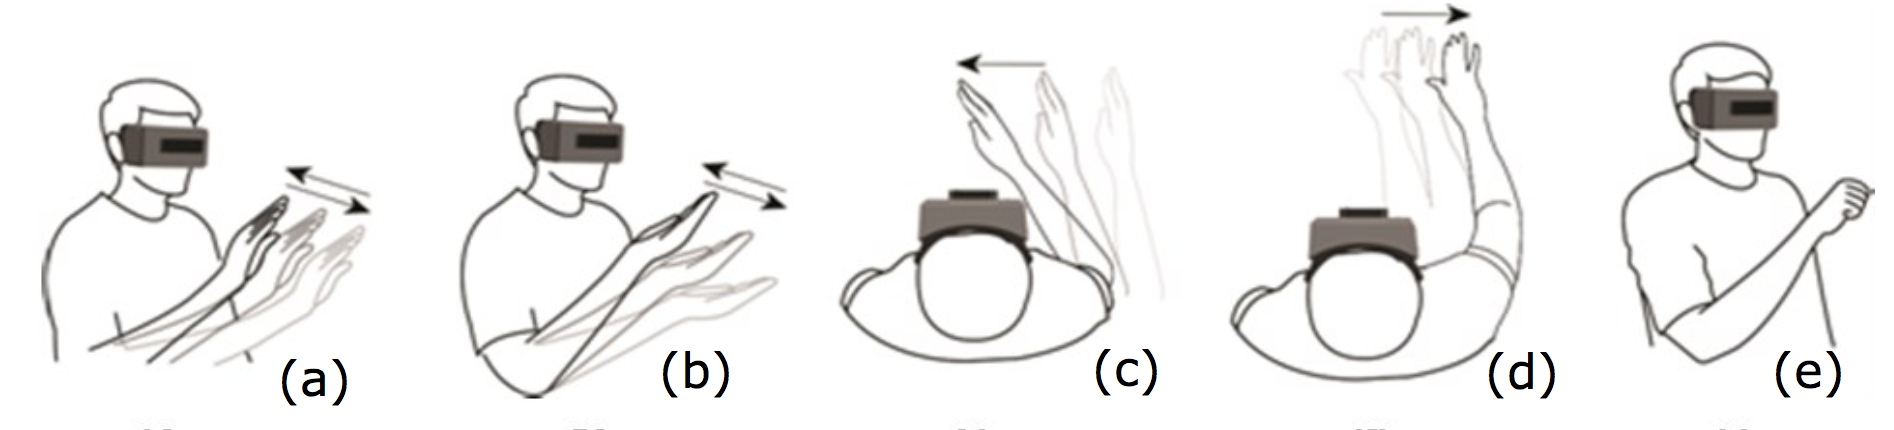
\includegraphics[width=14cm]{03_Figures/05_LitReview/Khundam2015_LeapMotion.png}
		\caption[Hand gestures for forward/backward movement, stepping left/right and holding position]{Hand gestures for forward/backward movement (a,b), stepping left/right (c,d) and holding position (e) \citep{Khundam2015}}
		\label{fig:leapmotion}
	\end{center}
\end{figure}
\newline
For their research on static and stroke gestures, \cite{Chun2015} made use of a depth-camera in order to track hand gestures and combined it with speech recognition. The latter is discussed in more detail in chapter \ref{SubSubSectionSpeechRecognition} which covers the methods of speech recognition in general. \cite{Chun2015} defined different hand and finger gestures for selecting, moving, scaling, rotating, copying and deleting objects, all of which actions had to be confirmed by a specific yes/no gesture. This set of gestures makes it a very natural, intuitive and interactive way for the user to alter virtual objects. As often with the use cameras, there are limitations to it. The hand has to be tracked properly for the whole performance of the gesture and it has to be done with the right speed for a proper recognition of the command \citep{Chun2015}.


\subsubsection{Gesture Controllers}

\label{SubSubSectionGestureControllers}

Very similar to the hand gestures, the gesture controllers intend to improve the tracking of the hand movements by adding hardware to the hands of the users that is easier to track but still leaves options for simple interaction with buttons and triggers. \newline
One of the first commercial gesture controllers was the \textit{PlayStation Move}, introduced by \cite{Sony2010}. While the controller itself can detect its own motion, the position is tracked with a camera attached to the PlayStation. This allows for a more accurate tracking of a specific point which \cite{Takala2014} made use of by attaching a PlayStation Move to their HMD in order to have a more accurate positioning than it was possible with solely the Microsoft Kinect. \newline
Alongside the \textit{HTC Vive} HMD, a new gesture controller also have been introduced \citep{Htcvive2016}. In combination with the Lighthouse technology (described in chapter \ref{360MotionTracking}), the controllers can also be properly tracked if they are e.g. hidden behind the back of the user, which is not possible with the PlayStation Move. Figure \ref{fig:gesturecontroller} shows this controller with its unique design for the tracking sensors (6) and a combination of track-pad (2), buttons (1, 3 and 8) and a trigger (7). By putting the thumb on the track-pad, the index finger on the trigger and the other three fingers on the side button it almost allows to track the grabbing motion of the hand.
\begin{figure}[h]
	\begin{center}
		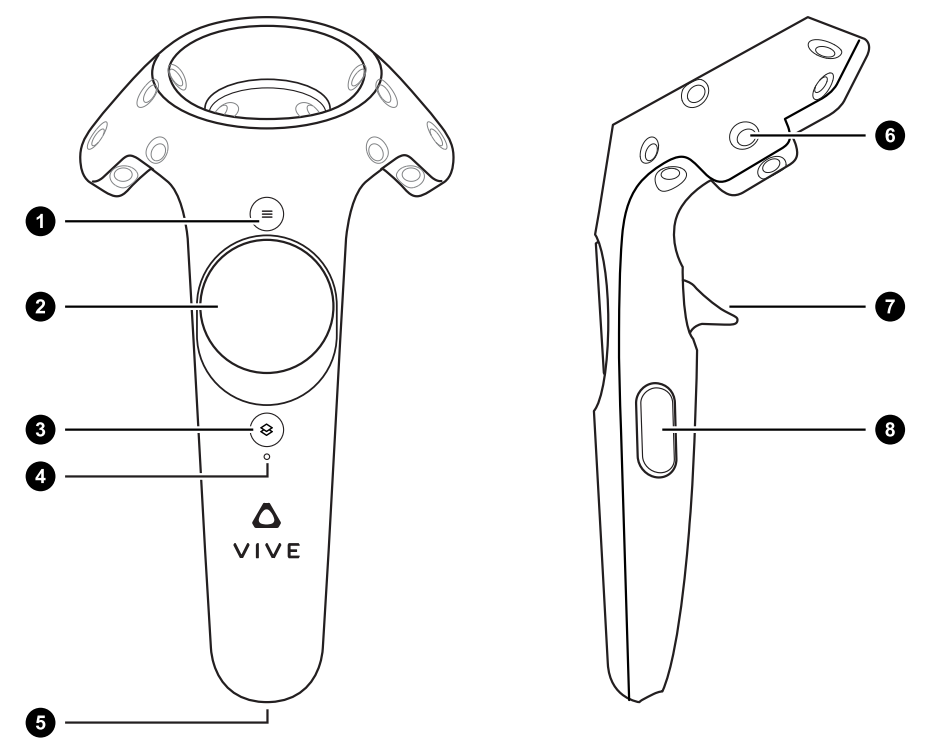
\includegraphics[width=10cm]{03_Figures/05_LitReview/HTCCorp2016_GestureController.png}
		\caption[Gesture Controller for the HTC Vive]{Gesture Controller for the HTC Vive \citep{HTCCorp2016}}
		\label{fig:gesturecontroller}
	\end{center}
\end{figure}


\subsubsection{Speech Recognition}

\label{SubSubSectionSpeechRecognition}

The second natural interaction after hand gestures is speech recognition It is often combined with hand gesture as they can complement each other quite seamlessly. \newline
For the navigation within 3D scans from \gls{mri} or \gls{ct}, \cite{Muller1998} proposed a speech recognition system as illustrated with an example in Figure \ref{fig:speechrecognitionmedical}. With semantic decoding and a semantic structure, the commands can be interpreted and processed by the intention decoder to tell the system what to do \citep{Muller1998}. This is a very time-consuming process since all commands have to be prepared and acoustic-phonetic models need to be generated during the collection of training data. Provided the users followed the instructions, a 99.8\% semantic accuracy could be achieved which basically means that the system is almost fully accurate in this scenario \citep{Muller1998}.
\begin{figure}[h]
	\begin{center}
		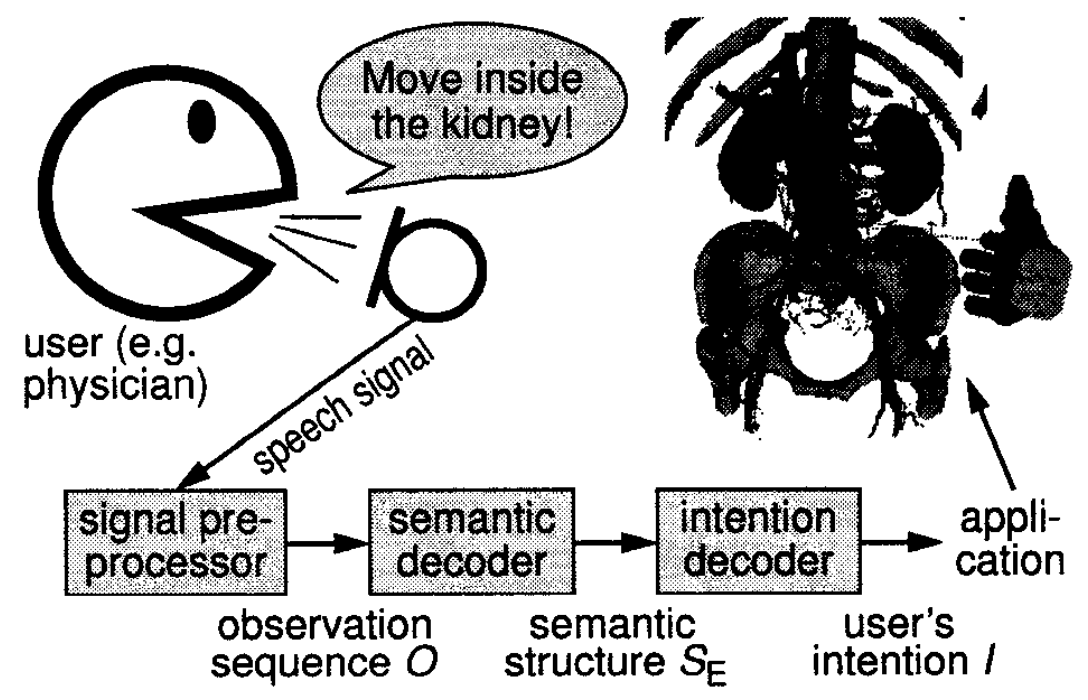
\includegraphics[width=10cm]{03_Figures/05_LitReview/Muller1998_SpeechRecognition.png}
		\caption[Architecture and example of speech recognition and interaction for physicians]{Architecture and example of speech recognition and interaction for physicians \citep{Muller1998}}
		\label{fig:speechrecognitionmedical}
	\end{center}
\end{figure}
\newline
\cite{Uchino2008} combined speech recognition with a camera to identify where the user is pointing at on a computer screen to interact with a virtual agent. In their example, a set of pens with different colours are presented to the user where the selection is made in combination with gestures (pointing at the pen) and speech (e.g. "\textit{Please give the red one}") \citep{Uchino2008}. Figure \ref{fig:speechrecignitionpen} shows how such a conversation with a virtual agent can proceed where the agent picks the wrong pen based on the pointing and ambiguous speech and thus has to be corrected to pick the one with the right colour Although this research was not focussed on virtual reality, this research can also be applied in virtual reality which might even improve the accuracy of the pointing gesture.
\begin{figure}[h]
	\begin{center}
		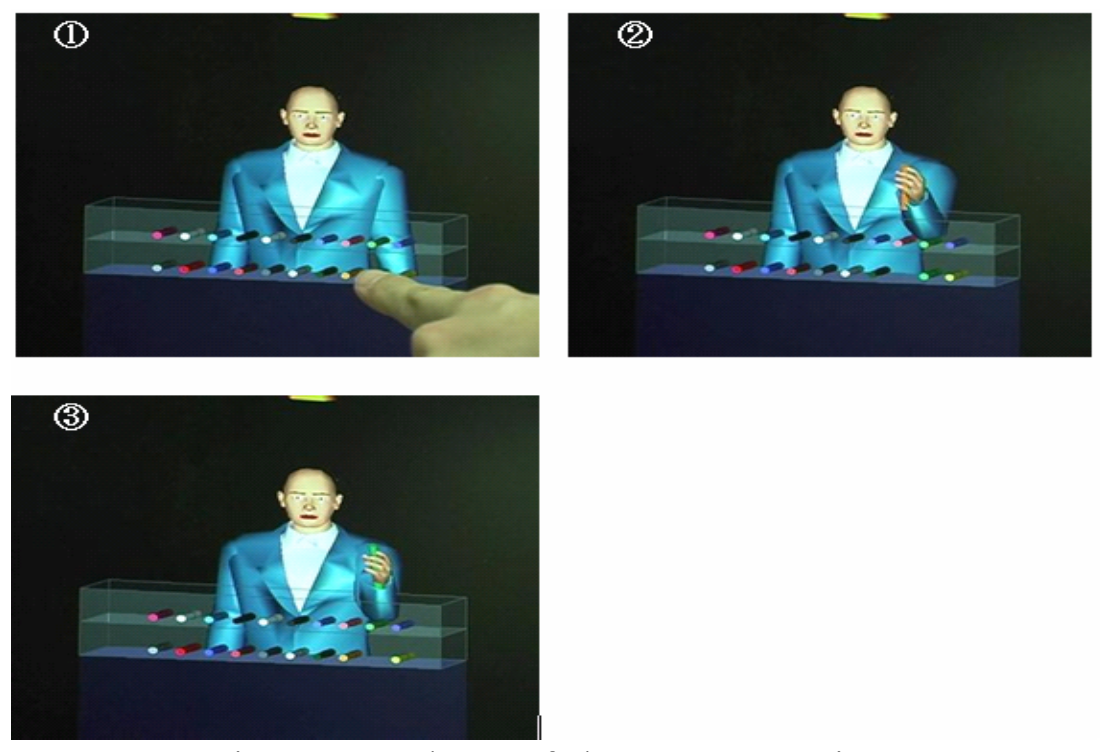
\includegraphics[width=10cm]{03_Figures/05_LitReview/Uchino2008_SpeechPointing.png}
		\caption[Flow of a conversation with the virtual pen agent]{Flow of a conversation with the virtual pen agent \citep{Uchino2008}}
		\label{fig:speechrecignitionpen}
	\end{center}
\end{figure}
\newline
As described in chapter \ref{SubSubSectionHandGestures}, \cite{Chun2015} utilized hand gestures to interact with virtual objects and further enhanced them with speech recognition. While objects can be altered in their spatial appearance, speech is used to change the colour of the object or ask questions about the type, shape or colour of it \citep{Chun2015}. Instead of relying on a physical device with buttons to change the colours, a multi-modal interaction combines speech and gesture to a more natural and intuitive method that is also closer to the real world \citep{Chun2015} .


\subsubsection{Physical Placement of Interactive Objects}

Quite a bit older, from the 1990s, is the idea of dynamically placing physical knobs and switches in front of a seated user wearing a HMD \citep{Latham1997}. The trajectory of the users hand and its movement is extrapolated in order to move the correct type of control in the right position just when it is expected in the virtual reality environment \citep{Latham1997}. Figure \ref{fig:touchcockpit} shows the concept of \cite{Latham1997} as well as how the final design looked like. Since such a machine requires a lot of time to design and build, it can be assumed that these are parts of the reason why not many further advancements were undertaken.
\begin{figure}[h]
	\begin{center}
		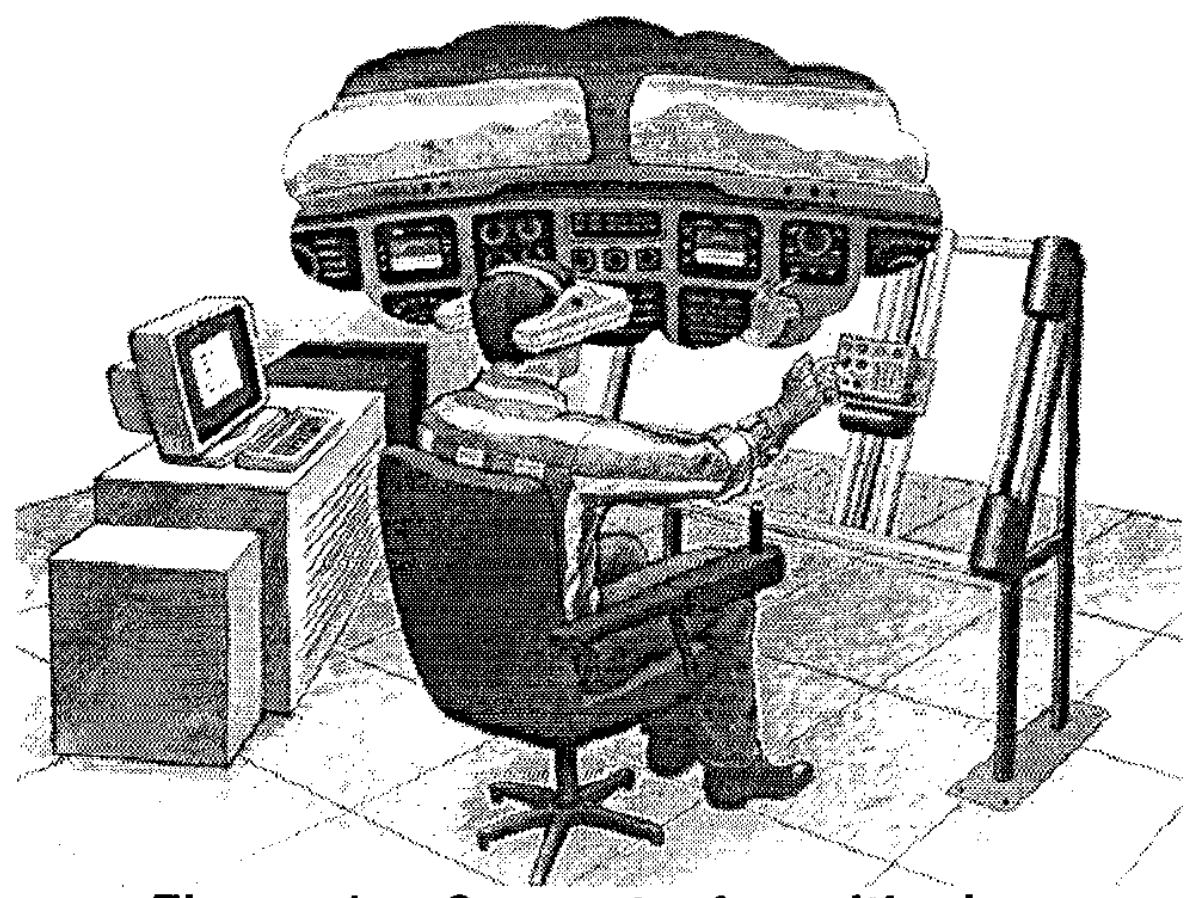
\includegraphics[width=6cm]{03_Figures/05_LitReview/Latham1997_Concept.png}
		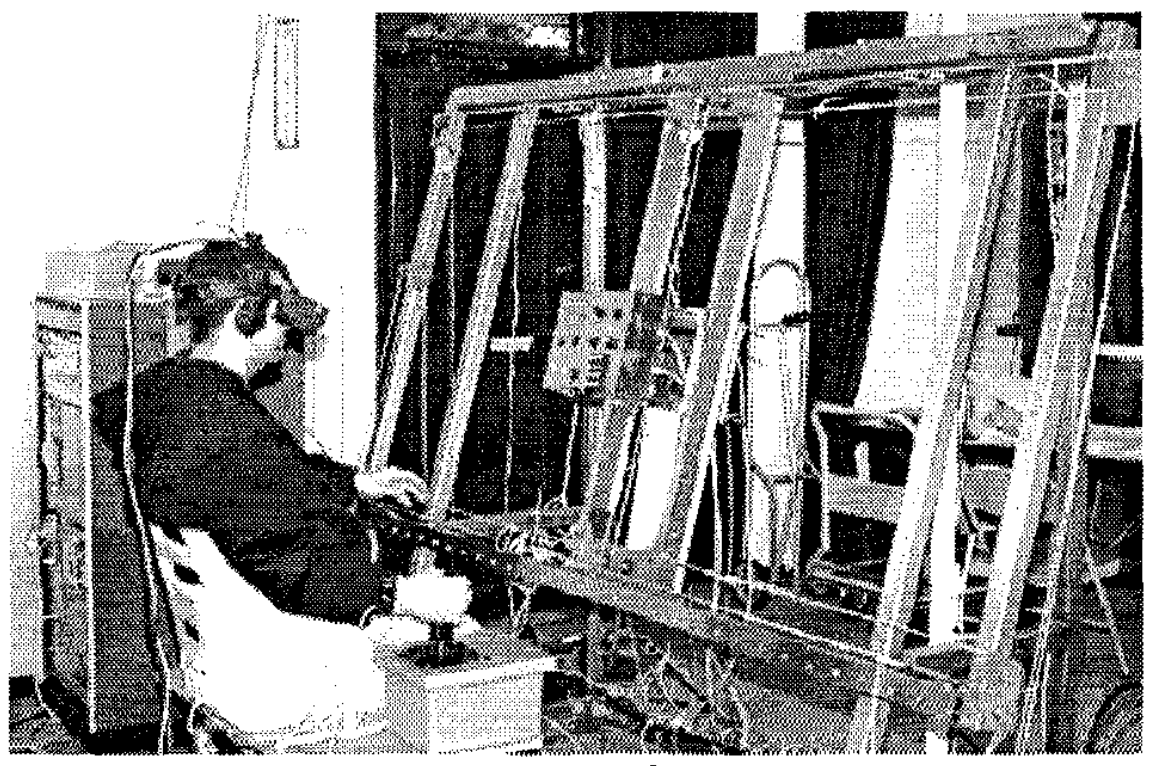
\includegraphics[width=7cm]{03_Figures/05_LitReview/Latham1997_FinalDesign.png}
		\caption[Concept and final design of positioning instrument controls to be touched in a virtual cockpit]{Concept (left) and final design (right) of positioning instrument controls to be touched in a virtual cockpit \citep{Latham1997}}
		\label{fig:touchcockpit}
	\end{center}
\end{figure}


\subsubsection{Full Body Tracking}

In June 2010, Microsoft announced the \textit{Kinect for Xbox 360}, a controller-free gaming device for the living room \citep{Microsoft2010}. Instead of relying on any physical input devices, the Kinect contains a camera with motion-sensing technology that can track up to 48 points of movement on the human body, turning the player himself into a controller \citep{Microsoft2010}. \newline
Based on this technology, \cite{Takala2014} proposed a combination of a full body avatar controlled by Kinect with the Oculus Rift as display. This combination proved to be quite powerful although they were facing a couple of challenges as well. The Kinect sometimes lost track of the hands or the movement was not recognized at all which \cite{Takala2014} tried to resolve by attaching a PlayStation Move to the HMD and put a Razer Hydra controller into the hands (Figure \ref{fig:kinectbody}). Although this improved the situation, different latencies of the individual devices dampened the experience. Furthermore, although Kinect was used for full-body tracking, only the movement of the hands and legs was utilized, whereas the movement within the virtual world was still relying on a physical controller.
\begin{figure}[t]
	\begin{center}
		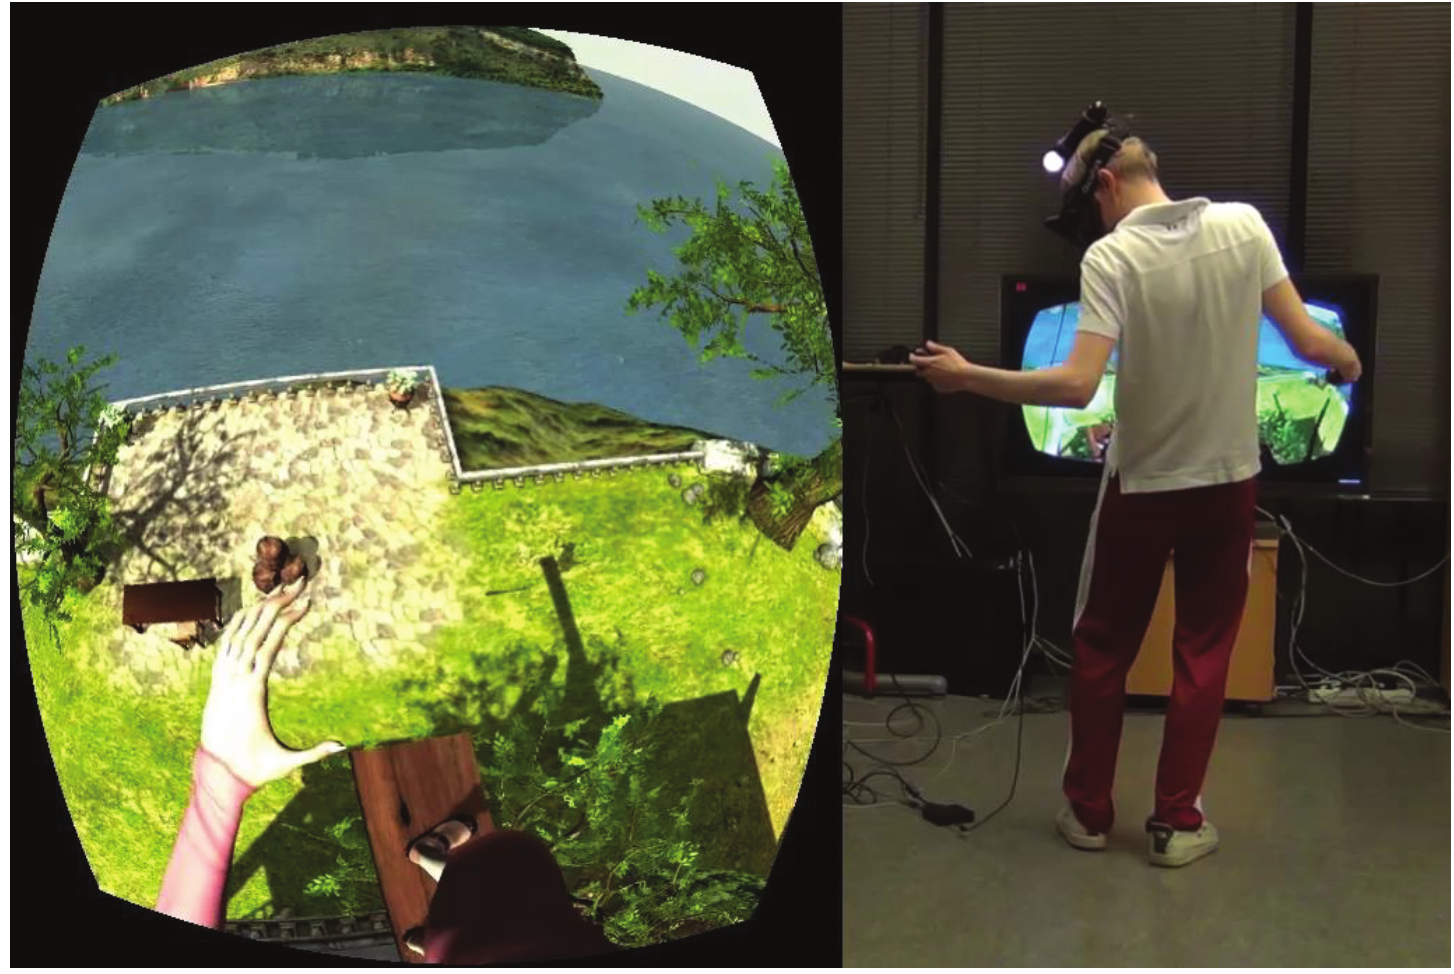
\includegraphics[width=12cm]{03_Figures/05_LitReview/Takala2014_KinectBody.png}
		\caption[Player's view of their virtual body that is tracked with Kinect]{Player's view of their virtual body (left) that is tracked with Kinect (right) \citep{Takala2014}}
		\label{fig:kinectbody}
	\end{center}
\end{figure}


\subsubsection{360° Motion Tracking}
\label{360MotionTracking}

One of the latest additions to the interaction possibilities is the 360° motion tracking, introduced with the HTC Vive which was just released in April 2016 \citep{Htcvive2016}. Figure \ref{fig:lighthouses} shows the setup of the two base stations (i.e. Lighthouses) in opposing corners of the room that will be used for the 360° motion tracking. In essence, the two Lighthouse base stations emit a laser sweep across the room 60 times a second with a flash in between which allows any device with photo-sensors to calculate its exact position relative to the base station(s) \citep{Gizmodo2015}. This allows for a very accurate tracking and due to the opposing corners, at least one Lighthouse always has direct \textit{line of sight} to the HMD and the controllers. \newline
With this additional sensor information, the movement of the HMD and the controllers is tracked in all three axis and allows for new movements to be recognized, such as crouching or jumping within the relations of the room.
\begin{figure}[h]
	\begin{center}
		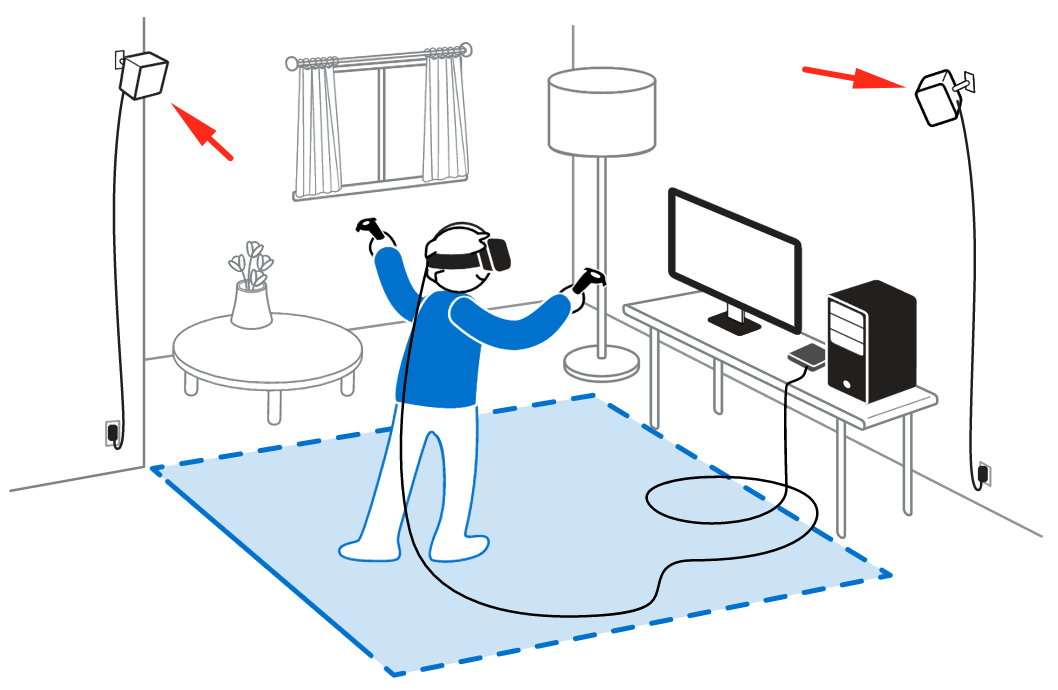
\includegraphics[width=10cm]{03_Figures/05_LitReview/HTCCorp2016_LighthouseRoomScale.png}
		\caption[Two Lighthouse in opposing corners allow for 360° motion tracking]{Two Lighthouse in opposing corners allow for 360° motion tracking \citep{HTCCorp2016}}
		\label{fig:lighthouses}
	\end{center}
\end{figure} \newline
A more simplified variation of this is described by \cite{Donalek2014}, who used a ViconTM motion-capturing system with infrared markers on the HMD to track its spatial location. This allowed \cite{Donalek2014} to also recognize movements such as kneeling down or looking over and around objects in the scene, however always limited by the volume that was covered by the Vicon system. \newline
The main difference to full body tracking is that the 360° motion tracking relies on physical sensors to derive their (i.e. the sensors) position within three dimensional space compared to the detection of any movable object (usually the body of a person). This method is much more accurate than the full body tracking, but requires additional hardware to do so.


%-----------------------------------
%	SUBSECTION 3
%-----------------------------------

\subsection{Conclusion}

The literature review on different methods for user input in virtual reality showed that there are various types which can be used or even combined. \newline
There are six main methods for user input in virtual reality. These are hand gestures, gesture controllers, speech recognition, physical placement of interactive objects, full body tracking and 360° motion tracking. Hand gestures track the movement of the whole hand and/or the individual fingers with one or more (regular, infra-red or depth) cameras. Gesture controllers are physical devices with buttons that are held in the hands and also tracked in their spatial position. Speech recognition tries to understand and interpret spoken words and sentences in order to find the correct commands. The physical placement of interstice objects extrapolates the movement of the hand to physically place a button in front of the finger where a virtual one is shown in \gls{vr}. Full body tracking uses cameras to track the whole body including the movement of all extremities from one angle. Finally, 360° motion tracking can locate the position of special devices within an actual room on all three axis from opposing corners. The most used method in the reviewed literature is the hand gestures, followed by the hand gestures in combination with speech recognition \newline
Depending on the chosen method, there are advantages and disadvantages (or even limitations) for certain use cases. Table \ref{tbl:methodscomparison} shows a summary of these findings and is also the answer to the first \gls{srq}.
\begin{table}[h]
	\begin{center}
		\begin{tabular}{ | p{3.7cm} | p{4.9cm} | p{4.9cm} | }
			\hline
			\textbf{Method} & \textbf{Advantages} & \textbf{Disadvantages} \\
			\hline
			Hand Gestures & 
			- Highest familiarity \newline - Inexpensive & 
			- Limited tracking area \newline - Only from one angle \newline - Decreasing accuracy with faster movement  \\
			\hline
			Gesture Controllers &
			- Very accurate \newline - Similarity to hand gestures \newline - Buttons for more interaction &
			- Additional device required \newline - Have to be held all the time \\
			\hline
			Speech Recognition &
			- Most natural to humans \newline - Known from smartphones &
			- Different languages, dialects \newline - Requires silent area \\ 
			\hline
			Physical Placement of Objects &
			- Realistic experience \newline - Tangible interaction with \gls{vr} &
			- Expensive \newline - Difficult to build \newline - Stationary \\ 
			\hline
			Full Body Tracking &
			- Tracks all extremities \newline - Natural interaction possible &
			- Only from one angle \newline - Limited accuracy on details \\ 
			\hline
			360° Motion Tracking &
			- Room-scale movement \newline - Very accurate \newline - Spatial positioning on all three axis &
			- Only dedicated HMD and controllers can be tracked \newline - Stationary (base stations) \\ 
			\hline
		\end{tabular}
		\caption{Advantages and disadvantages/limitations of different methods for user input in virtual reality}
		\label{tbl:methodscomparison}
	\end{center}
\end{table} \newline
In regards of the thesis statement, a combination of two methods is recommended to outweigh the individual disadvantages and utilize the benefits of both methods.


%----------------------------------------------------------------------------------------
%	SECTION 2
%----------------------------------------------------------------------------------------

\section{Existing Interaction Patterns in Virtual Reality}

\label{SectionLiteratureReviewSRQ2}

This chapter addresses the second \gls{srq} by having a look at existing interaction patterns in virtual reality and evaluating their strengths and weaknesses. It starts with a short introduction, followed by an analysis of the visual information seeking mantra. Then more details are given on different interaction patterns for travel, selection and manipulation as well as the idea of multi-modal interaction, before the importance of immersion and task performance is elaborated. A conclusion summarizes the research done in this chapter.
\begin{framed}
	\textit{\gls{srq} 2: \srqtwotext}
\end{framed}

%-----------------------------------
%	SUBSECTION 1
%-----------------------------------

\subsection{Introduction}

During the 1960s, the first interaction patterns such as clicking or grabbing and moving objects have been defined on which even now we are still relying on with mouse and keyboard \citep{Myers1998}. But with wearing a \gls{hmd}, the situation changes as it obstructs our view on the so well known devices. New methods for user input had to be researched and inherently also new interaction patterns had to be defined. \cite{Donalek2014} mentioned that a new tool is required where physical gestures can be used to manipulate with virtual objects. In order to understand what kind of gestures should be considered, the Visual Information Seeking Mantra of \cite{Shneiderman1996} is looked at.


%-----------------------------------
%	SUBSECTION 2
%-----------------------------------

\subsection{Visual Information Seeking Mantra}

\label{SubSectionVISM}

\cite{Shneiderman2005} defined a set of principles for direct manipulation, amongst which are:
\begin{itemize}[noitemsep,nolistsep]
	\item visual representation of the world of action including both the objects and actions
	\item rapid, incremental and reversible actions
	\item selection by pointing (instead of typing)
\end{itemize}
Based on this, \cite{Ahlberg1994} proposed the Visual Information Seeking Principle in 1994 that focused in displaying a graph with buttons and sliders for real-time manipulation of the displayed data. This concept fulfilled all principles for direct manipulation and was so successful that it became the foundation for the \gls{vism} \citep{Shneiderman1996}. \cite{Shneiderman1996} was looking at many visual design guidelines but fundamentally always concluded the following mantra:
\begin{framed}
	\textit{Overview first, zoom and filter, then details-on-demand}
\end{framed}
As an abstraction of reality, \cite{Shneiderman1996} further defined seven tasks (four main and three support tasks) that are inherently crucial for the analysis and work with data.

Main tasks:
\begin{itemize}[noitemsep,nolistsep]
	\item Overview \textit{(Gain an overview of the entire collection)}
	\item Zoom \textit{(Zoom in on items of interest)}
	\item Filter \textit{(Filter out uninteresting items)}
	\item Details-on-demand \textit{(Select and item or group and get details when needed)}
\end{itemize}
Support tasks:
\begin{itemize}[noitemsep,nolistsep]
	\item Relate \textit{(View relationships among items)}
	\item History \textit{(Keep a history of actions to support undo, replace and refinement)}
	\item Extract \textit{(Allow extraction of sub-collections and of the query parameters)}
\end{itemize}
Figure \ref{fig:vism} shows a visualisation of these tasks as well as the relationship to each other. It shows that in order to move from the \textit{Overview} to the \textit{Details}, the user either has to \textit{Zoom} or apply some \textit{Filtering} on the presented data set.
\begin{figure}[h!]
	\begin{center}
		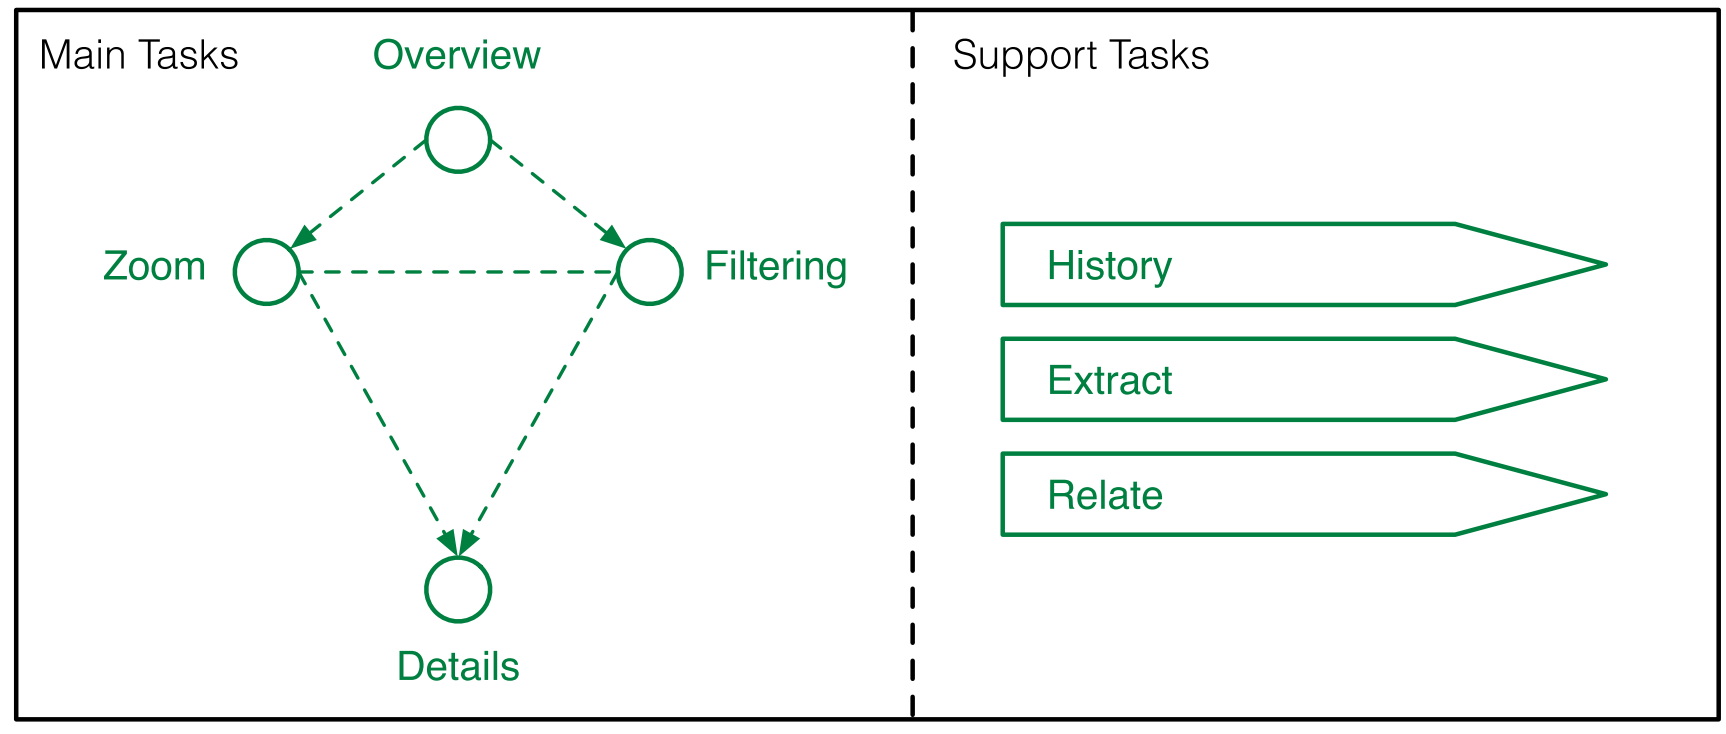
\includegraphics[width=12cm]{03_Figures/05_LitReview/Stauffer2016_VISM1.png}
		\caption[Visual Information Seeking Mantra]{Visual Information Seeking Mantra \citep{Stauffer2016}}
		\label{fig:vism}
	\end{center}
\end{figure} \newline
\cite{Stauffer2016} reviewed and extended the \gls{vism} to version 2.0. By distinguishing between \textit{Zoom In} and \textit{Zoom Out} as well as allowing for a more flexible entry point for the different tasks, they also deal with one of the big downfalls of \gls{vism} when a user already knows what data is important and thus does not want to start with the \textit{Overview} \citep{Neil2006}. Shifting \textit{Relate} to the main tasks helps to align it with \textit{Details} to provide a multi view where multiples views can be shown and altered simultaneously \citep{Stauffer2016}. The additional \textit{Collaboration} support tasks suggest that communication possibilities should be implemented directly inside the the application system instead of relying on third party applications. Figure \ref{fig:vism2} shows version 2.0 of the \gls{vism} with a direct comparison of 1.0 (green) and 2.0 (orange). \newline
\begin{figure}[h!]
	\begin{center}
		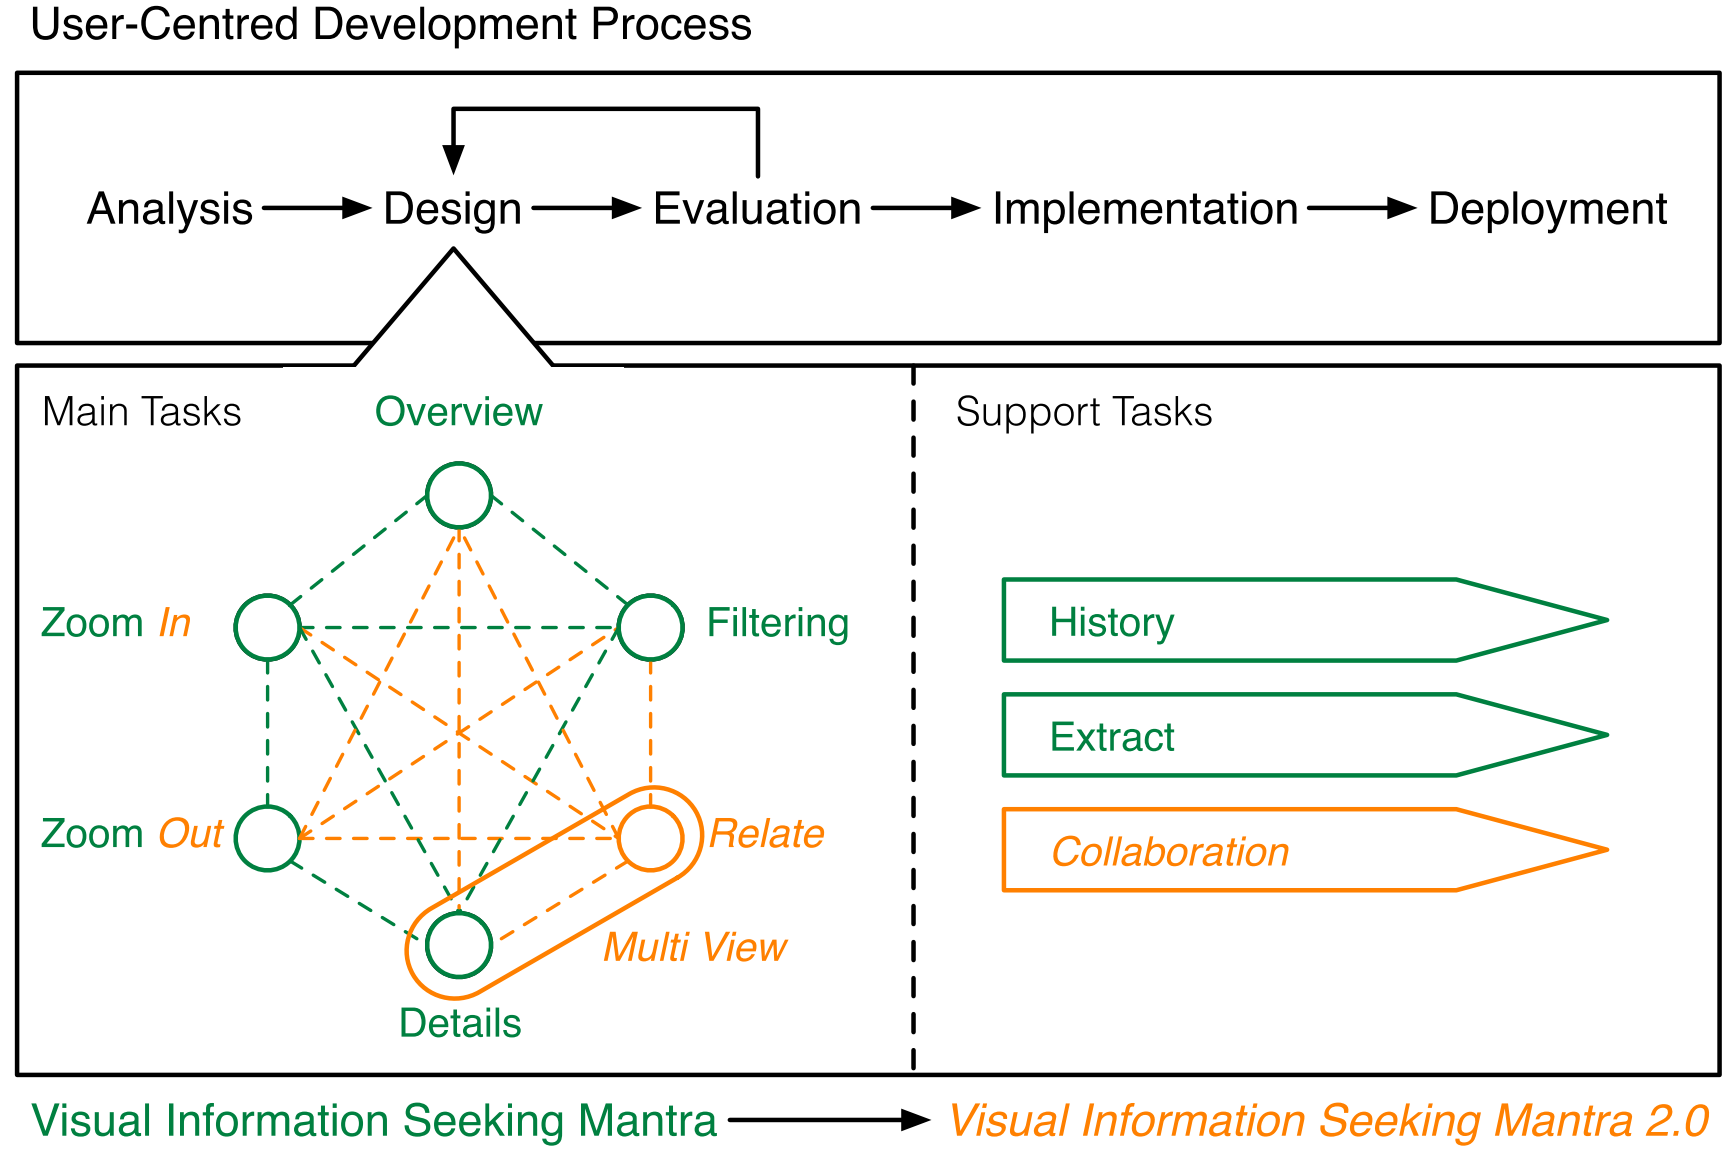
\includegraphics[width=12cm]{03_Figures/05_LitReview/Stauffer2016_VISM2.png}
		\caption[Visual Information Seeking Mantra 2.0]{Visual Information Seeking Mantra 2.0 \citep{Stauffer2016}}
		\label{fig:vism2}
	\end{center}
\end{figure}

In the analysis of \gls{vism} by \cite{Craft2005}, they point out that it should only be seen as guidelines and also note that although it defines some tasks that a system \textit{should} fulfil, it gives no indication on the question \textit{"How?"}. This conclusion can still be seen as valid since also with version 2.0 of the \gls{vism}, the focus remains on what kind of interaction should be present and not how these interactions could look like.


%-----------------------------------
%	SUBSECTION 3
%-----------------------------------

\subsection{Interaction Patterns}

\label{SubSectionInteractionPatterns}

\cite{Bunt1998} stated that "Human communication is inherently multimodal in nature". What he meant with this is that in a multi-modal user interface, a user can combine a spoken natural language request with one or more gestures \citep{Rosson2002}. By allowing this combination, the interaction in virtual reality can become closer to how we already interact with each other in real life. \newline
In order to understand the different interaction patterns better, \cite{Bowman2002} has grouped them in three distinctive categories: Travel, Selection and Manipulation. \textit{Travel} deals with how the user can navigate in the \gls{ve}, how the movement and visual exploration works. \textit{Selection} focuses on the first interaction with a virtual object, how one or many object can be selected and how this is visualized for the user. Finally, in \textit{Manipulation} the actual alteration of a virtual object in its appearance and behaviour is discussed.


%-----------------------------------
%	SUBSUBSECTION 1
%-----------------------------------

\subsubsection{Travel}

In \gls{vr}, the most important interaction pattern is the navigation itself, since without navigation the experience is not much different from a 2D display. \cite{Kwon2015} and \cite{Jamieson2007} confirmed in their research that the simplest method for this is to utilize the built in head tracking capabilities of the \gls{hmd} itself. It in fact is more familiar to us humans to examine objects of interest this way, rather than using mouse and keyboard \citep{Jamieson2007}. Either with the gyroscope sensor information or with tracking the position and direction of the camera, this information allows to determine where the user is looking at \citep{Kwon2015}. \cite{Jamieson2007} continue that for a totally immersive experience in \gls{vr}, also body movement would have to be tracked to allow to walk around or even to put the head inside the visualized data objects.

\cite{Deligiannidis2003} researched this topic based on a problem from practice where a person is working on a specific task in \gls{vr} and up to 20 outsider participants can observe and comment on the work of the fully immersed person. The use of vocal instructions however was distracting to everyone and there were no possibilities for the outsiders to interact with the \gls{ve} \citep{Deligiannidis2003}. Their solution to this was dividing the area in front of each outsider into two hemispheres, reaching with the hands in the top one allowed each person to manipulate the camera (third person view) whereas if the hands are on the lower one the hand manipulation (first person view) was activated \citep{Deligiannidis2003}. This combination allowed the before passive observers to be much more immersed in the \gls{ve} and to do exploration on their own.

During their demonstrations, \cite{Drouhard2015} observed difficulties when the users wearing a \gls{hmd} had to interact (blindly) with keyboard and mouse, whereas most of them could use an Xbox controller rather intuitively. In their application, the controller was used to "fly" around within the \gls{ve} and the head tracking capabilities of the \gls{hmd} allowed them to explore the environment and look at the data from different perspectives \citep{Drouhard2015}.

\cite{Bowman2002} also defined guidelines for designing travel techniques, which inherently are related to the navigation and can be summarized as follows:
\begin{itemize}[noitemsep,nolistsep]
	\item Make simple travel tasks simple by using target-based techniques
	\item Use physical head motion for viewpoint orientation if possible
	\item Avoid teleportation; provide smooth transitional motion between locations instead
	\item If steering techniques are used, users should be trained beforehand
	\item Use non-head-coupled techniques for efficiency in relative motion tasks
	\item Provide integrated aids to help the user decide where to move
\end{itemize}

The reviewed literature showed that for looking around, researchers exclusively relied on the head-tracking capabilities of the \gls{hmd} whereas for the travel in space either third-party controllers were used or the idea of full body tracking was briefly mentioned.

On a more practical side, \cite{CloudheadGames2016} released their \gls{vr} game \textit{The Gallery - Episode 1: Call of the Starseed} for the HTC Vive in April 2016 and offered two different ways for travelling in the \gls{ve}. The player can chose between "gaze-teleportation" where the location to be teleported at is controlled with the \gls{hmd} and confirmed with a click, or "point-teleportation" where the target spot is chosen and confirmed by pointing at with the gesture controller \citep{CloudheadGames2016}. While the travelling with gaze follows the research of \cite{Jamieson2007} and their conclusion that using the \gls{hmd} is the simplest method, it limits the possibilities for multitasking. By utilizing the gesture controllers for travelling, a certain independence of the viewing experience is achieved and allows "blind" travelling without the need to also look into that direction, just like if we walk backwards in the real world. Both methods of travelling are illustrated in Figure \ref{fig:gazePointTeleportation}.
\begin{figure}[h]
	\begin{center}
		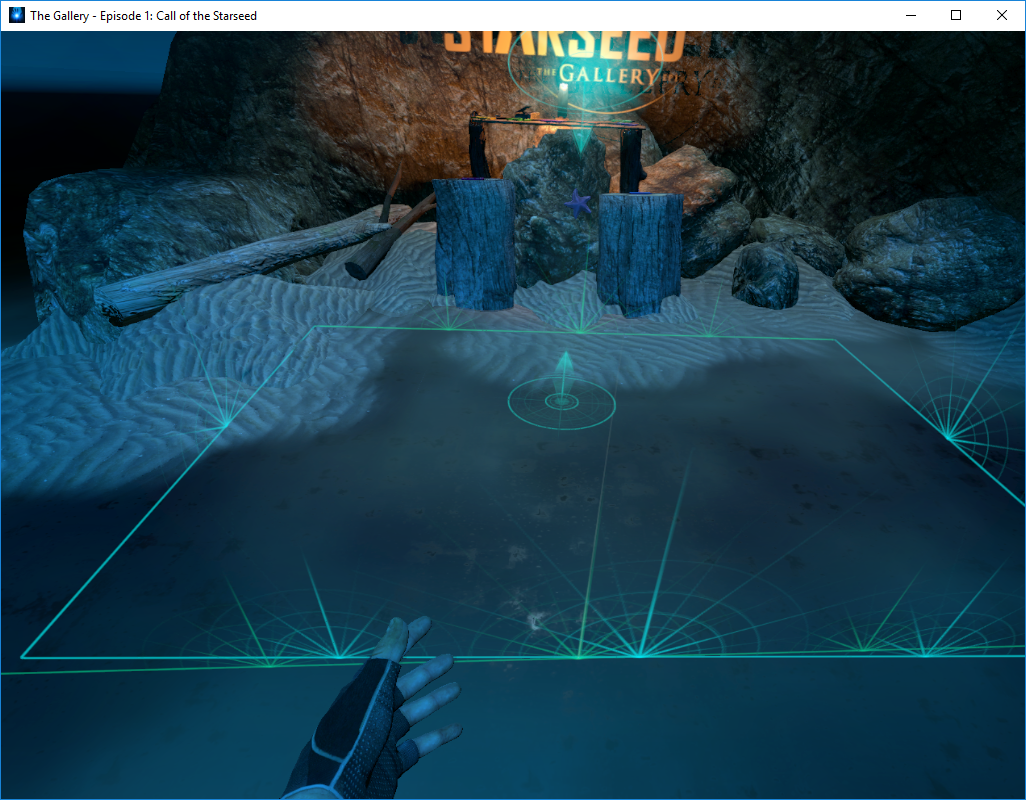
\includegraphics[width=7cm]{03_Figures/05_LitReview/Cloudhead2016_TheGallery2.png}
		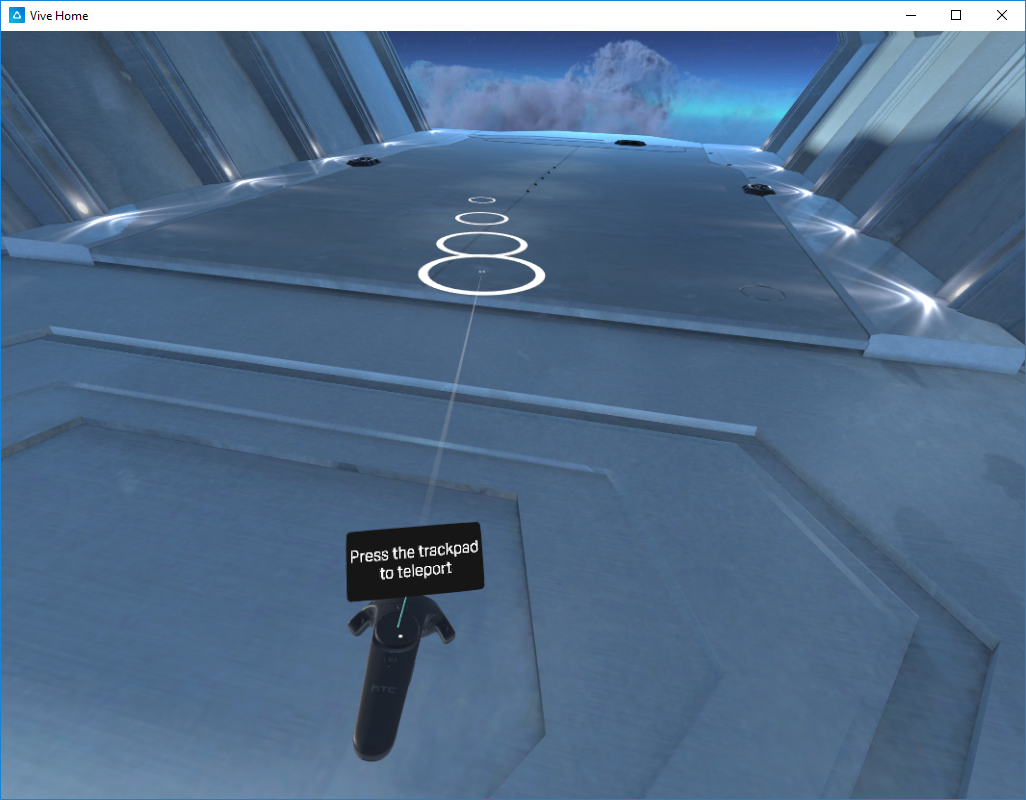
\includegraphics[width=7cm]{03_Figures/05_LitReview/HTCVive2016_ViveHome.png}
		\caption[Gaze and point teleportation in "The Gallery" and "Vive Home"]{Gaze (left) and point (right) teleportation in "The Gallery"  \citep{CloudheadGames2016} and "Vive Home" \citep{Htcvive2016a}}
		\label{fig:gazePointTeleportation}
	\end{center}
\end{figure} \newline
The fact that both options are provided for the player to chose from can be seen as an indication, that even in practice for entertainment purposes, there is no clear strategy yet as to which travelling method is more natural, efficient or practical.

%-----------------------------------
%	SUBSUBSECTION 2
%-----------------------------------

\subsubsection{Selection}

After looking at \textit{Travel}, the second interaction pattern is the selection of objects in the \gls{ve} either to get more information on them or to do manipulate them in a subsequent step. Based on the selected input method, different patterns come to action. \newline
\cite{Bowman2002} also defined guidelines for designing selection techniques that can be summarized as follow:
\begin{itemize}[noitemsep,nolistsep]
	\item Use the natural virtual hand technique if all selection is within arm's reach
	\item Use ray-casting techniques if speed of remote selection is a requirement
	\item The chosen selection technique should integrates well with the manipulation technique
	\item Multi-modal input for combined selection and command tasks
	\item Environment design should maximize the perceived size of objects
	\item Provide integrated aids to help the user decide where to move
\end{itemize}

Research showed, that three main types of selection patterns have been research: Hand, HMD Reticle and Gesture Controllers.

\subparagraph{Hand}

\cite{Steed2006} researched different simple selection techniques using the hand. He distinguishes between Ray-based selection, Small Volume Selection and Cone Selection which are illustrated in Figure \ref{fig:selectiontechniques} \citep{Steed2006}. In the Ray-based selection, an imaginary ray is cast in the direction of the hand to choose the first object interacts with (object A), whereas in the Small Volume selection, the intersection of the hand with the volume of an object determines the selection (object C) \citep{Steed2006}. Lastly, \cite{Steed2006} defined the Cone Selection similar to the Ray-based one, however there are two rays in this case and all objects that are in between them are considered selected (objects E and F). \newline
Each technique has different applications where it makes more sense or allows for a better immersion than any of the other techniques, such as when a virtual button or handle can be triggered, the Small Volume selection can be considered the closest to how we would interact in the real world. \newline
Since these techniques are highly linked to the methods of using hand gestures as input, they bring their strengths and weaknesses along. While it is the most familiar way for humans to interact (or in this case to select something), it is highly depending on accurate tracking capabilities and good interpretation of gestures if more than a simple pointing gesture is required.
\begin{figure}[h]
	\begin{center}
		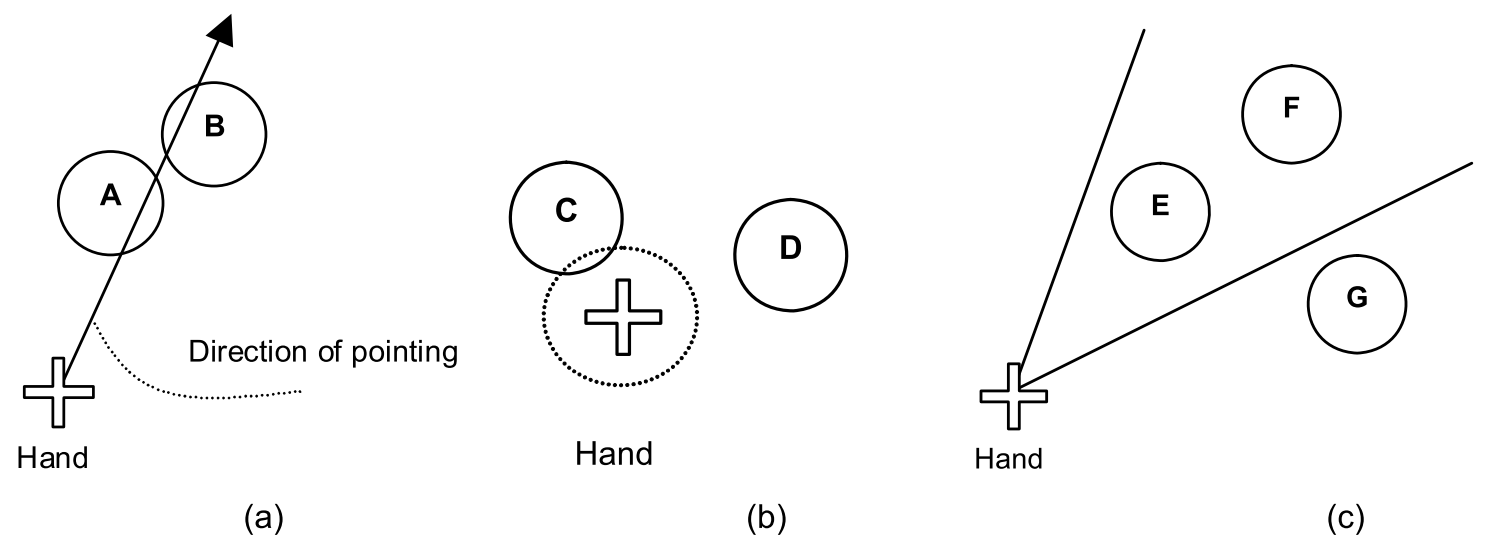
\includegraphics[width=14cm]{03_Figures/05_LitReview/Steed2006_SelectionTechniques.png}
		\caption[Simple selection techniques for objects in \gls{vr}: Ray-based, Small Volume Selection and Cone Selection]{Simple selection techniques for objects in \gls{vr}: Ray-based (a), Small Volume Selection (b) and Cone Selection (c) \citep{Steed2006}}
		\label{fig:selectiontechniques}
	\end{center}
\end{figure}


\subparagraph{HMD Reticle}

\cite{Kwon2015} and \cite{Drouhard2015} focused their research on a selection technique using a reticle that is visualized inside the \gls{hmd}, like a cross-hair. When the user selects a node with this reticle, this node and its neighbours are brought closer to the user and are highlighted in order to see more details and allow the user to make further selections \citep{Kwon2015}. With the option to select multiple nodes and the visualization of the nodes amongst themselves, interesting paths or relations can be visualized in an effective way \citep{Kwon2015}. It however is not mentioned how the selection itself is triggered, whether a button has to be pushed or if the gaze just has to be held for a couple of seconds. It is also not mentioned how the "\textit{Zoom Out}" task can be performed. \newline
\cite{Drouhard2015} provided more details on this part in their research where they implement a "target mode" that the user can enter. Only in this case the cross-hair reticle is shown to the user and the selection happens by targeting a data object and pressing the trigger button \citep{Drouhard2015}. It can be assumed that this separation of "target mode" and "view mode" will help the combination of \textit{Selection} and \textit{Travel} and makes the data analysis more convenient as the reticle is only shown when absolutely necessary. \newline
\cite{Drouhard2015} furthermore states that gaze interaction arguably is the most natural form of interaction in \glspl{ve}. \newline
One fact that is not mentioned in literature but becomes clear is that with an \gls{hmd} reticle, the selection is directly linked to the viewing experience. It is not possible to select something without directly looking at it, which inherently limits the multitasking possibilities.


\subparagraph{Gesture Controller}

\label{HentschelFigureRef}

Finally, also gesture controllers allow for dedicated selection patterns. \cite{Hentschel2009} used a controller to select multiple data points out of a 3D scatter-plot which they called interactive brushing and is shown in Figure \ref{fig:interactivebrushing}. The first (left) picture shows the empty selection box that can be moved and scaled (middle and right picture) in order to make the actual selection \citep{Hentschel2009}. Although the middle and right picture look almost the same, the difference is that with the middle picture the visualization of the scatter-plot is done in real-time and only upon releasing the button on the device, the actual selection with remote selection and computing is done \citep{Hentschel2009}.
\begin{figure}[h]
	\begin{center}
		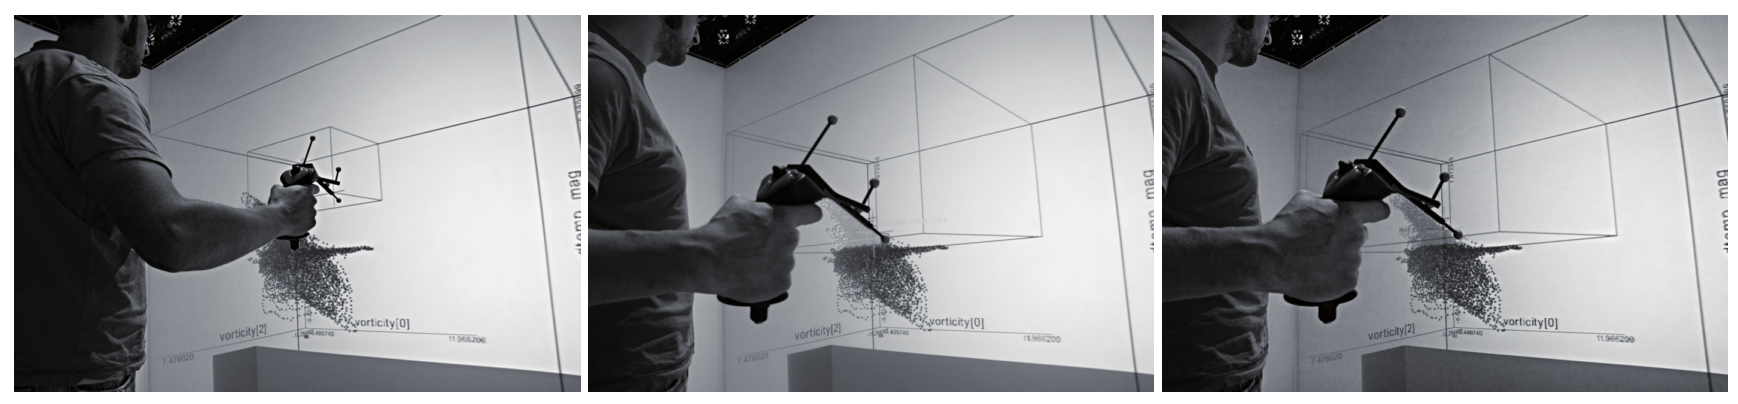
\includegraphics[width=14cm]{03_Figures/05_LitReview/Hentschel2009_InteractiveBrushing.png}
		\caption[Box selection of scatter-plot data in \gls{vr}]{Box selection of scatter-plot data in \gls{vr} \citep{Hentschel2009}}
		\label{fig:interactivebrushing}
	\end{center}
\end{figure} \newline
In their game \textit{The Gallery - Episode 1: Call of the Starseed}, \cite{CloudheadGames2016} provide the option to select objects by utilizing the gesture controllers that in \gls{vr} are visualized as hands as shown in Figure \ref{fig:theGalleryHands}. With the trigger button, the hand can be closed and thus objects can be grabbed and moved around. The game further distinguishes between "important" and "unimportant" objects, where the "important" ones are stuck in the grip of the hand even if the trigger was released (i.e. a flashlight) and "unimportant" objects would immediately drop once the trigger button is released. This allows for a more convenient interaction since it can become irritating to keep the trigger button held for a longer amount of time. \newline
\begin{figure}[h]
	\begin{center}
		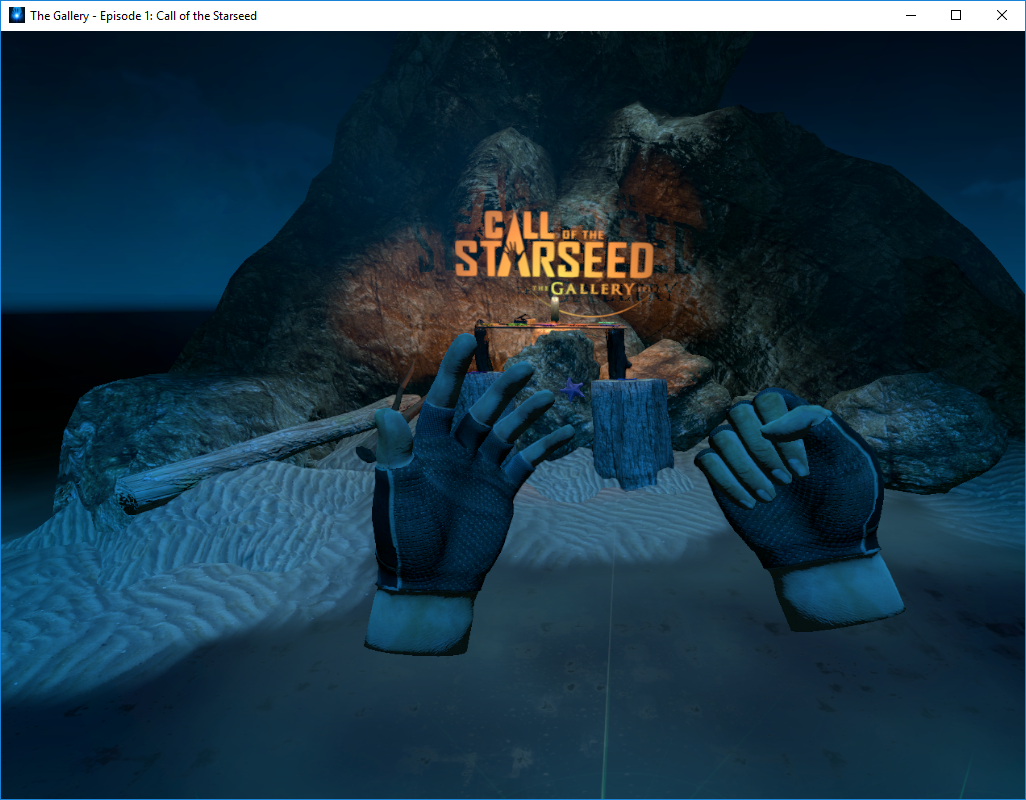
\includegraphics[width=7cm]{03_Figures/05_LitReview/Cloudhead2016_TheGallery.png}
		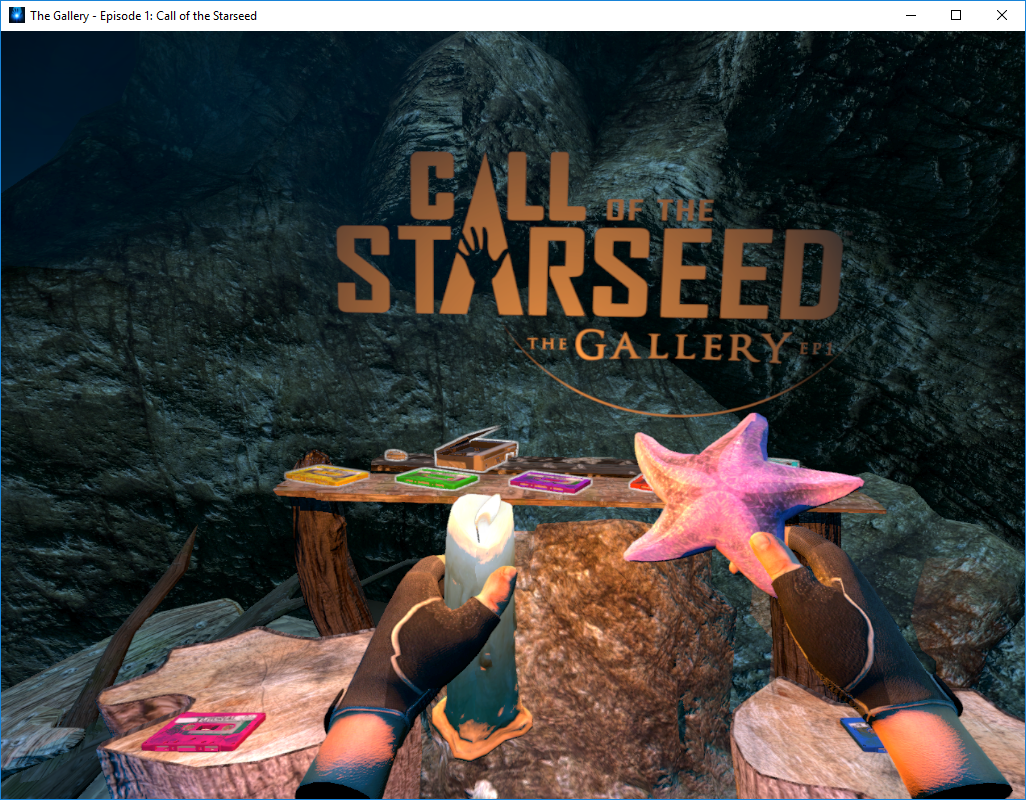
\includegraphics[width=7cm]{03_Figures/05_LitReview/Cloudhead2016_TheGallery3.png}
		\caption[Gesture Controllers visualized as Hands in "The Gallery"]{Gesture Controllers visualized as Hands in "The Gallery" \citep{CloudheadGames2016}}
		\label{fig:theGalleryHands}
	\end{center}
\end{figure} \newline
As with the selection by hand, also the selection by gesture controllers brings their advantages and disadvantages from the method as an input device itself with them. While they offer very good accuracy and increased functionality with buttons and triggers, it requires additional hardware and tracking devices.


%-----------------------------------
%	SUBSUBSECTION 3
%-----------------------------------

\subsubsection{Manipulation}

As early as in the 1980s, interaction patterns with data (i.e. manipulations) have already been defined, such as the "Put-That-There" voice and gesture interface as described by \cite{Bolt1980}. This interfaces focus on certain voice command to manipulate objects in a virtual space which have been defined as following \citep{Bolt1980}:
\begin{itemize}[noitemsep,nolistsep]
	\item "Create..." \textit{(a default object, with default size and colour on a default position)}
	\item "Move..." \textit{(an object to a specific position)}
	\item "Make that..." \textit{(altering an object in colour and size)}
	\item "Delete..." \textit{(removal of an object)}
	\item "Call that..." \textit{(give an object a name to which it can be referred to)}
\end{itemize}
In addition, the spoken \textit{"there"} serves as some kind of voice button where the \textit{"there"} refers to the cursor position, thus introducing the gestures as an input method for this interface \citep{Bolt1980}.
It can be seen that even more than three decades ago, the need to simplify more complicated interactions such as changing the colour of an object, which would require several inputs actions with mouse or keyboard, were tested to be simplified with new means of interaction patterns. \cite{Donalek2014} also mentioned the need for a new tool where the user can manipulate with these objects since wearing a \gls{hmd} blocks the view on the keyboard interface. \newline
\cite{Woodard2015} explained their approach on a more technical level in which they basically utilized the concept of the Small Volume Selection from \cite{Steed2006} to trigger certain manipulations like opening a door (i.e. rotating an object on its axis).

\cite{Bowman2002} again defined guidelines for designing manipulation techniques, that can be summarized as follow:
\begin{itemize}[noitemsep,nolistsep]
	\item Provide constraints (general or specific) or manipulation aids
	\item Allow direct manipulation with the virtual hand instead of using a tool
	\item Avoid repeated, frequent scaling of the user or environment
	\item Use indirect depth manipulation for increased efficiency and accuracy
\end{itemize}

Literature review has shown that most research focuses on \textit{Travel} and \textit{Selection} whereas \textit{Manipulation} of data objects is in most cases not covered at all. This is also shown with the defined guidelines from \cite{Bowman2002} as they are more vague than for the other techniques.

With the release of the HTC Vive, \cite{Google2016} released a \gls{vr} application called \textit{Tilt Brush} which basically is a 3D painting application in virtual reality. It allows the user to choose between different pencils, brush sizes, colours and also provides an "undo" functionality, all that is controlled with pop-up menus that can be interacted with using the gesture controllers as shown in Figure \ref{fig:tiltBrushMenus}.
\begin{figure}[h]
	\begin{center}
		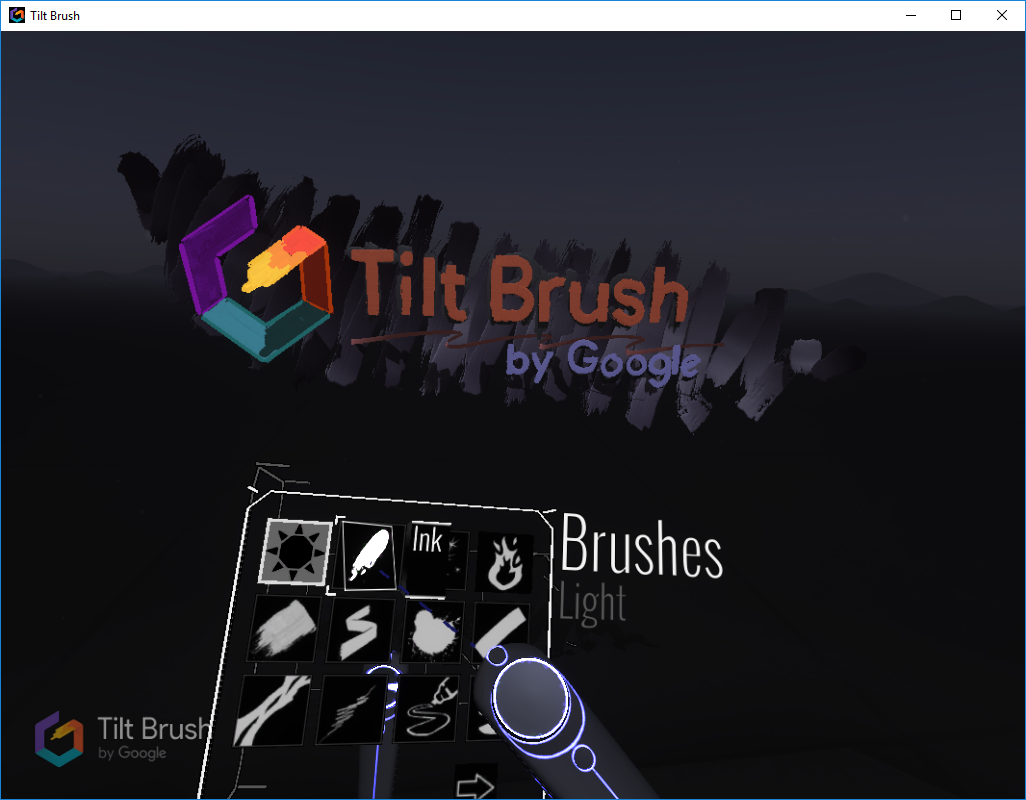
\includegraphics[width=7cm]{03_Figures/05_LitReview/Google2016_TiltBrush.png}
		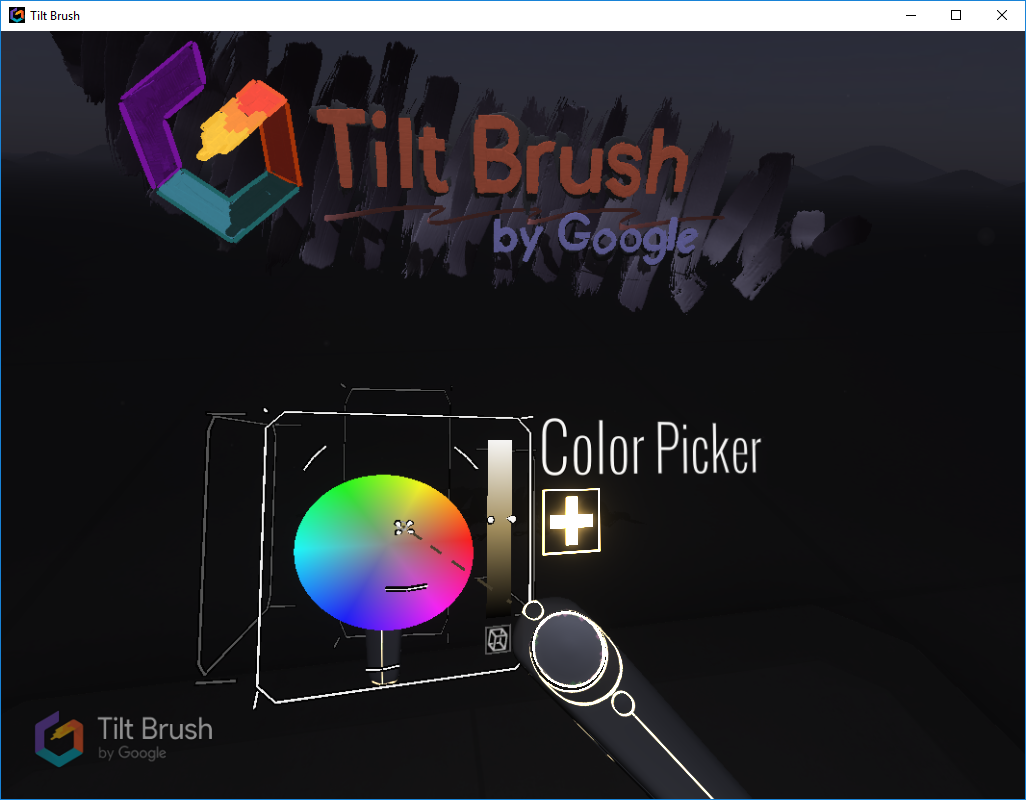
\includegraphics[width=7cm]{03_Figures/05_LitReview/Google2016_TiltBrush2.png}
		\caption[Pop-up menu with Gesture Controllers in "Tilt Brush"]{Pop-up menu with Gesture Controllers in "Tilt Brush" \citep{Google2016}}
		\label{fig:tiltBrushMenus}
	\end{center}
\end{figure} \newline
The research of \cite{Bowman2002} has shown, that this type of non-natural interaction indeed can be quite effective, especially since it allows for tasks to be executed that cannot be done naturally. Although it would be possible to provide a virtual colour palette where the user would have to choose the colour by hand to eliminate this option from the pop-up menu, this would drastically impact the task performance in a negative way.


%-----------------------------------
%	SUBSECTION 4
%-----------------------------------

\subsection{Importance of Immersion and Task Performance}

In addition to the interaction patterns to perform tasks, the level of immersion and the performance of task execution is as important. \cite{Woodard2015} defined three rules a project has to be conform with in order to be as immersive as possible:
\begin{itemize}[noitemsep,nolistsep]
	\item Three Dimensional Viewing
	\item Full User-Navigation Integration
	\item Interactive Environment
\end{itemize}
The first two points have to be ensured by the application design itself as well as interaction patterns for \textit{Travel}. The third point is more complex as it covers the interaction patterns for \textit{Selection} and \textit{Manipulation} which are more crucial for the performance.

\cite{Bowman2002} separates the term performance a bit more and considers two aspects of it:
\begin{itemize}[noitemsep,nolistsep]
	\item Task performance \textit{(quality of task completion, measured in time, accuracy, ...)}
	\item Technique performance \textit{(qualitative experience of the user during interaction)}
\end{itemize}
Since the technique performance is ultimately related to the concept of usability, which is not part of this thesis, the main focus lies on the task performance.

\cite{Bowman2002} continues that it is a common misconception that in order to be an effective \gls{ve}, it should behave and work as close to the real world as possible; interaction should be "natural". \cite{Smith1987} called this naturalistic approach "\textit{Naturalism}" whereas the addition of non-natural methods he simply called "\textit{Magic}". The possibility to scale objects or create them out of thin air, to be able to fly around in space are considered to be magic techniques \citep{Bowman2002}. There are also more simple 2D objects such as drop-downs, pop-up menus or buttons that are already widely spread in our everyday applications that we use on computers and smartphones. \cite{Bowman2002} concludes that although these techniques are less natural and might even require some training, if designed for specific interaction tasks, they can be more efficient and flexible than any natural technique.\newline
\cite{Rosson2002} looked at immersion a bit different and summarized it as an "all around" experience for the user which requires multi-modal input (e.g. data gloves or speech recognition) and output (e.g. \gls{hmd} or haptic feedback on a device). The degree to which someone fells like actually being "in" this \gls{ve} is depending on the available inputs and outputs and is often referred to as presence \citep{Rosson2002}.\newline
It can be said that if a task feels tedious and difficult to execute in \gls{vr}, it will have a difficult time to keep people interested in it, after all it should help us to become more efficient in our task performance.


%-----------------------------------
%	SUBSECTION 6
%-----------------------------------

\subsection{Conclusion}

The \gls{vism} provides a solid foundation of what tasks the interaction patterns should be able to fulfil. It however gives no guidelines or recommendations in how these interaction patterns could look like. The interaction patterns can be grouped into three categories: \textit{Travel}, \textit{Selection} and \textit{Manipulation}. Each of them has its own patterns which are more or less suited for certain applications. In general it can be seen that the \textit{Manipulation} pattern are researched the least so far and can be a suitable candidate for further research. Whichever interaction pattern is selected and implemented, its ability to allow the user to have a good task performance is crucial for any practical applications. \newline
In general, the strengths and weaknesses of the individual patterns are heavily related to advantages and disadvantages of the input method they base on. It can be said that the interaction patterns have to be selected in correlation with the decision for the matching input methods. Table \ref{tbl:pattermethodmapping} shows a mapping of pattern and method.
\begin{table}[t]
	\begin{center}
		\begin{tabular}{ | p{4cm} | p{6cm} | } 
			\hline
			\textbf{Interaction Pattern} & \textbf{Input Method} \\
			\hline
			Travel:  \newline \textit{Controllers} &
			- Gesture Controllers \newline - Physical Placement of Objects \\
			\hline
			Travel: \newline \textit{Full body tracking} &
			- Fully Body Tracking \newline - 360° Motion Tracking \\
			\hline
			Selection: \newline \textit{Hand} & 
			- Hand Gestures \\
			\hline
			Selection: \newline \textit{HMD Reticle} &
			- \gls{hmd} \\
			\hline
			Selection: \newline \textit{Gesture Controllers} &
			- Gesture Controllers \\ 
			\hline
			Manipulation: \newline \textit{"Put that there"} &
			- Speech Recognition \newline - Hand Gestures \\ 
			\hline
			Manipulation: \newline \textit{Others} &
			- Gesture Controllers \\ 
			\hline
		\end{tabular}
		\caption{Mapping of interaction pattern with their correlating input method}
		\label{tbl:pattermethodmapping}
	\end{center}
\end{table}

Although no distinct answer can be given to the second \gls{srq}, in combination with the findings from the first \gls{srq} it has been shown where the strengths lie and how they can be utilized. This also shows the close connection between the input method and interaction pattern and that they have to be aligned in order to create an immersive and productive experience.


%----------------------------------------------------------------------------------------
%	SECTION 3
%----------------------------------------------------------------------------------------

\section{Data Visualization}

\label{SectionLiteratureReviewSRQ3}

After covering the different methods for user input in \gls{vr} in chapter \ref{SectionLiteratureReviewSRQ1} and the interaction patterns in \gls{vr} in chapter \ref{SectionLiteratureReviewSRQ2}, this chapter concludes the literature research by looking at traditional data visualisation that are used for 2D data and how they have been applied to and enhanced for 3D space in \gls{vr}. After a short introduction to the topic with some theoretical background, several VR applications are analysed with a focus on data visualisation and data manipulation/interaction. Finally, the research covered in this chapter is summarized in the conclusion and will answer the third \gls{srq}.
\begin{framed}
	\textit{\gls{srq} 3: \srqthreetext}
\end{framed}


%-----------------------------------
%	SUBSECTION 1
%-----------------------------------

\subsection{Introduction}

With the invention of (multiple) windows on a computer screen in the late 1960s and the first spreadsheet (VisiCalc) developed in the late 1970s, the era for the visualization of data had just begun \citep{Myers1998}. Although the first \gls{hmd} was already invented in 1960 by Morton Heilig, it was only used for non-interactive film without any motion tracking \citep{vrs2015}. The actual availability for the public of such devices was not possible until the early 1990s although they still were rather expensive or did not fulfil the consumers expectations rendering them a flow (e.g. Nintendo Virtual Boy) \citep{vrs2015}. \cite{Ribarsky1994} highlighted that complicated manipulations of data will be simplified as \gls{vr} can provide a more natural interface between human and computer. He further continues that with \gls{vr} more of our senses are engaged than with regular 2D displays and thus can provide an opportunity to combine them \citep{Ribarsky1994}. \cite{Jamieson2007} further confirm the increased effectiveness and more natural and intuitive view on objects that use a 3D approach as it represents how humans view objects. \newline
\citet[p.411]{Stone1994} emphasized that: \blockquote{Visualization is more of a technique than a task. That is, people don't usually visualize data just for the hell of it.} They further conclude that due to the different goals for the visualization (e.g. testing a theory or understanding the data set), it makes it difficult on a general level to discuss the problems with how the visualization should be supported \citep{Stone1994}. This highlights the importance of the right type of visualization depending on the data itself and the goal that shall be reached. 


%-----------------------------------
%	SUBSECTION 2
%-----------------------------------

\subsection{Background Information}

For a better understanding of the specific applications, some theoretical background on data presentation and data manipulation/interaction is provided in the next two sub-chapters.

%-----------------------------------
%	SUBSUBSECTION 1
%-----------------------------------

\subsubsection{Data Presentation}

When we talk about the presentation of data, many will immediately think of Microsoft Excel and the many different charts (e.g. bar chart, line chart, pie chart, scatter plot etc.) that can be created with just a few clicks based on almost any data set. But not only in such mass consumer products, also big \gls{bi} solutions like \cite{TableauSoftware2016} rely on these well known and widely accepted techniques for their visualization of (big) data. Although multiple linked views have shown to be a good solution for interactive analysis of time-dependent data, one major short-coming when limited to a standard desktop-based setup is that complex spatial relationships are hard to understand when the data is only a 2D projection \citep{Hentschel2009}. \newline
\cite{Jamieson2007} highlighted that in the current time the focus shifted from producing and storing even larger amounts of data, to actually making use of it, especially since it becomes increasingly difficult to get a meaningful understanding of the data. They further continue that our traditional visualizations methods will come at their limits with the many different forms of (big) data that are produced every day \citep{Jamieson2007}. Also \cite{Sarathy2000} mentioned that with better performing hardware and software, more data can be collected and processed and thus going beyond the ability of humans to understand and comprehend this vast amounts of data with our traditional visualization methods. \cite[p.609]{Donalek2014} summarize this situation with \blockquote{Visualization is the main bridge between the quantitative content of the data and human intuition [...]} and that we arguably can only understand anything that can be visualized in some way. While it is possible to visualize a 3D object on a 2D display, \cite{Laha2012} see that it actually can become more difficult for the user to accurately judge the actual size, shape or depth of the volume data. Since an accurate understanding of the data is key, a visualisation with traditional displays might result in slower performance and/or wrong interpretation \citep{Laha2012}. This bears the questions whether \gls{vr} could be the enabling factor to surpass the current limitations of 2D visualization.\newline
\cite{VanDam2002} argue that with \gls{vr}, considerable advantages for non-human-scale visualizations can be achieved especially when the data should be explored in multiple spatial and temporal levels. To put this theory to a test, \cite{Ware1994} made a trial where the subjects had to look at a randomly organized network of nodes and arcs where two of the nodes where highlighted and they had to say whether these two nodes have a path between them. Based on their results, \cite{Ware1994} could conclude that compared to a 2D graph, with head coupled stereo the understood graphs were three times as large for any given error rate. \cite{Laha2012} also conducted a controlled empirical study to evaluate the effects of different levels of immersion, with the conclusion that while in general significant positive effects could be seen, it was also depending on the type of analysis task. This gives a strong indication on the potential benefits that can be achieved with the right visualization method in \gls{vr}.


%-----------------------------------
%	SUBSUBSECTION 2
%-----------------------------------

\subsubsection{Data Manipulation / Interaction}

\label{SubSectionVisualisationManipulation}

As stated by \cite{Stone1994}, people don't usually visualize data just for the visualisation's sake. It is at least as important what the goal of the visualization is and what the user should be able to do with it, i.e. how to move it around, twist it, shake it, change its colour mapping, expand it, rotate it, shrink it or slice and dice it \citep{Stone1994}. The direct manipulation of graphical objects has been in University Research since 1960, in Corporate Research since 1970 and in Commercial Products since 1980 \citep{Myers1998}. This shows that it was important from the beginning to be able to manipulate the data. Also \citet[p.410]{Stone1994} emphasized that: \blockquote{A visualization goal is to simplify the analysis of large-quantity, numerical data by rendering the data as an image that can be intuitively manipulated.} \cite{Stone1994} further continue to define three important characteristics that \gls{vr} has in this regard:
\begin{itemize}[noitemsep,nolistsep]
	\item \gls{vr} exhibits high interactivity (the user's actions and the caused reactions are tightly coupled together)
	\item \gls{vr} support embodiment (the user is represented  in the same spatial framework as the data)
	\item The \gls{vr} representation is spatial in nature (all virtual objects are placed in a spatial framework)
\end{itemize}
The first two characteristics give a clear indication how important it is that the user feels immersed inside the presented data and that his interactions with it are also updated visually. \cite{Jamieson2007} also mentions the importance of \gls{ve} allowing us to feel immersed within the 3D objects that represent the data. While the tracking of the users head position is an important start, \cite{Jamieson2007} define a totally immersive \gls{ve} as one where body movement is used to walk around and the users hand (real world) position is accurately mapped to the \gls{ve} to manipulate virtual objects. \cite{Drouhard2015} however also make aware of the fact, that especially in the case of scientific analysis, 2D visualisations have been used for decades and a transition to a 3D environment can be difficult, and thus focus should be put on how to bring the most effective 2D interactions into a 3D display. \newline
This leads to the first VR application that is focusing on a more traditional way of presenting data.


%-----------------------------------
%	SUBSECTION 3
%-----------------------------------

\subsection{Traditional Charts / Rotating Data Rings}

\label{SubSectionRotatingDataRings}

While any 2D chart can also be visualized in the same way in a \gls{ve}, it only can become beneficial when the additional space is utilized. \cite{Jamieson2007} mention the current possibilities of 2D mediums, such as desktop monitors, bring us to the limits of useful interactions and do not scale well anymore with large multi-dimensional data sets, wherefore new methods like \gls{vr} will be required. \cite{Jamieson2007} give an example where a data value can be represented as a 3D object, such as a box. This reminds of the 3D-like bar and pie charts from Microsoft Excel, except that they would be real 3D objects in three dimensional space instead of on a flat screen. \newline
\cite{Hentschel2009} was looking into creating a three-dimensional scatter plot in \gls{vr} as shown in Figure \ref{fig:interactivebrushing} in chapter \ref{HentschelFigureRef}. Within \gls{vr} it is possible here to make us of all three axis while the time-dependent data is handled with the animation of the scatter plot \citep{Hentschel2009}. While this could also be done on a 2D screen with the rotation of the data, the selection of multiple points is much simpler in \gls{vr} with the use of interactive brushing as mentioned by \cite{Hentschel2009}. \newline
A somewhat different approach to what we know as the bar charts has been presented by \cite{CodeScience2015} in their attempt to visualize sales data in a tower built from rotating data rings with varying speed that represent different products (as shown in Figure \ref{fig:rotatingringstoweranddetail}). Each ring is not fully closed and has a hole which helps to better compare the different rotational speeds whereas the different colours help to distinguish between the individual rings. In the demonstration of \cite{CodeScience2015}, the user as able to freely navigate (also vertically) around and inside the tower. When a data ring is selected, it expands and shows more detailed information (e.g. the different locations that sell the selected product) which again can be selected to narrow down the selection even further. In order to make use of the additional space in 3D and to present more relevant data together, \cite{CodeScience2015} displays the different information boxes in a circle around the user (as shown in Figure \ref{fig:rotatingringstoweranddetail}) and not just in front of him. This is quite an interesting approach and shows that visualization must not go completely different ways to provide a whole new experience in \gls{vr} for the presentation of data.
\begin{figure}[h]
	\begin{center}
		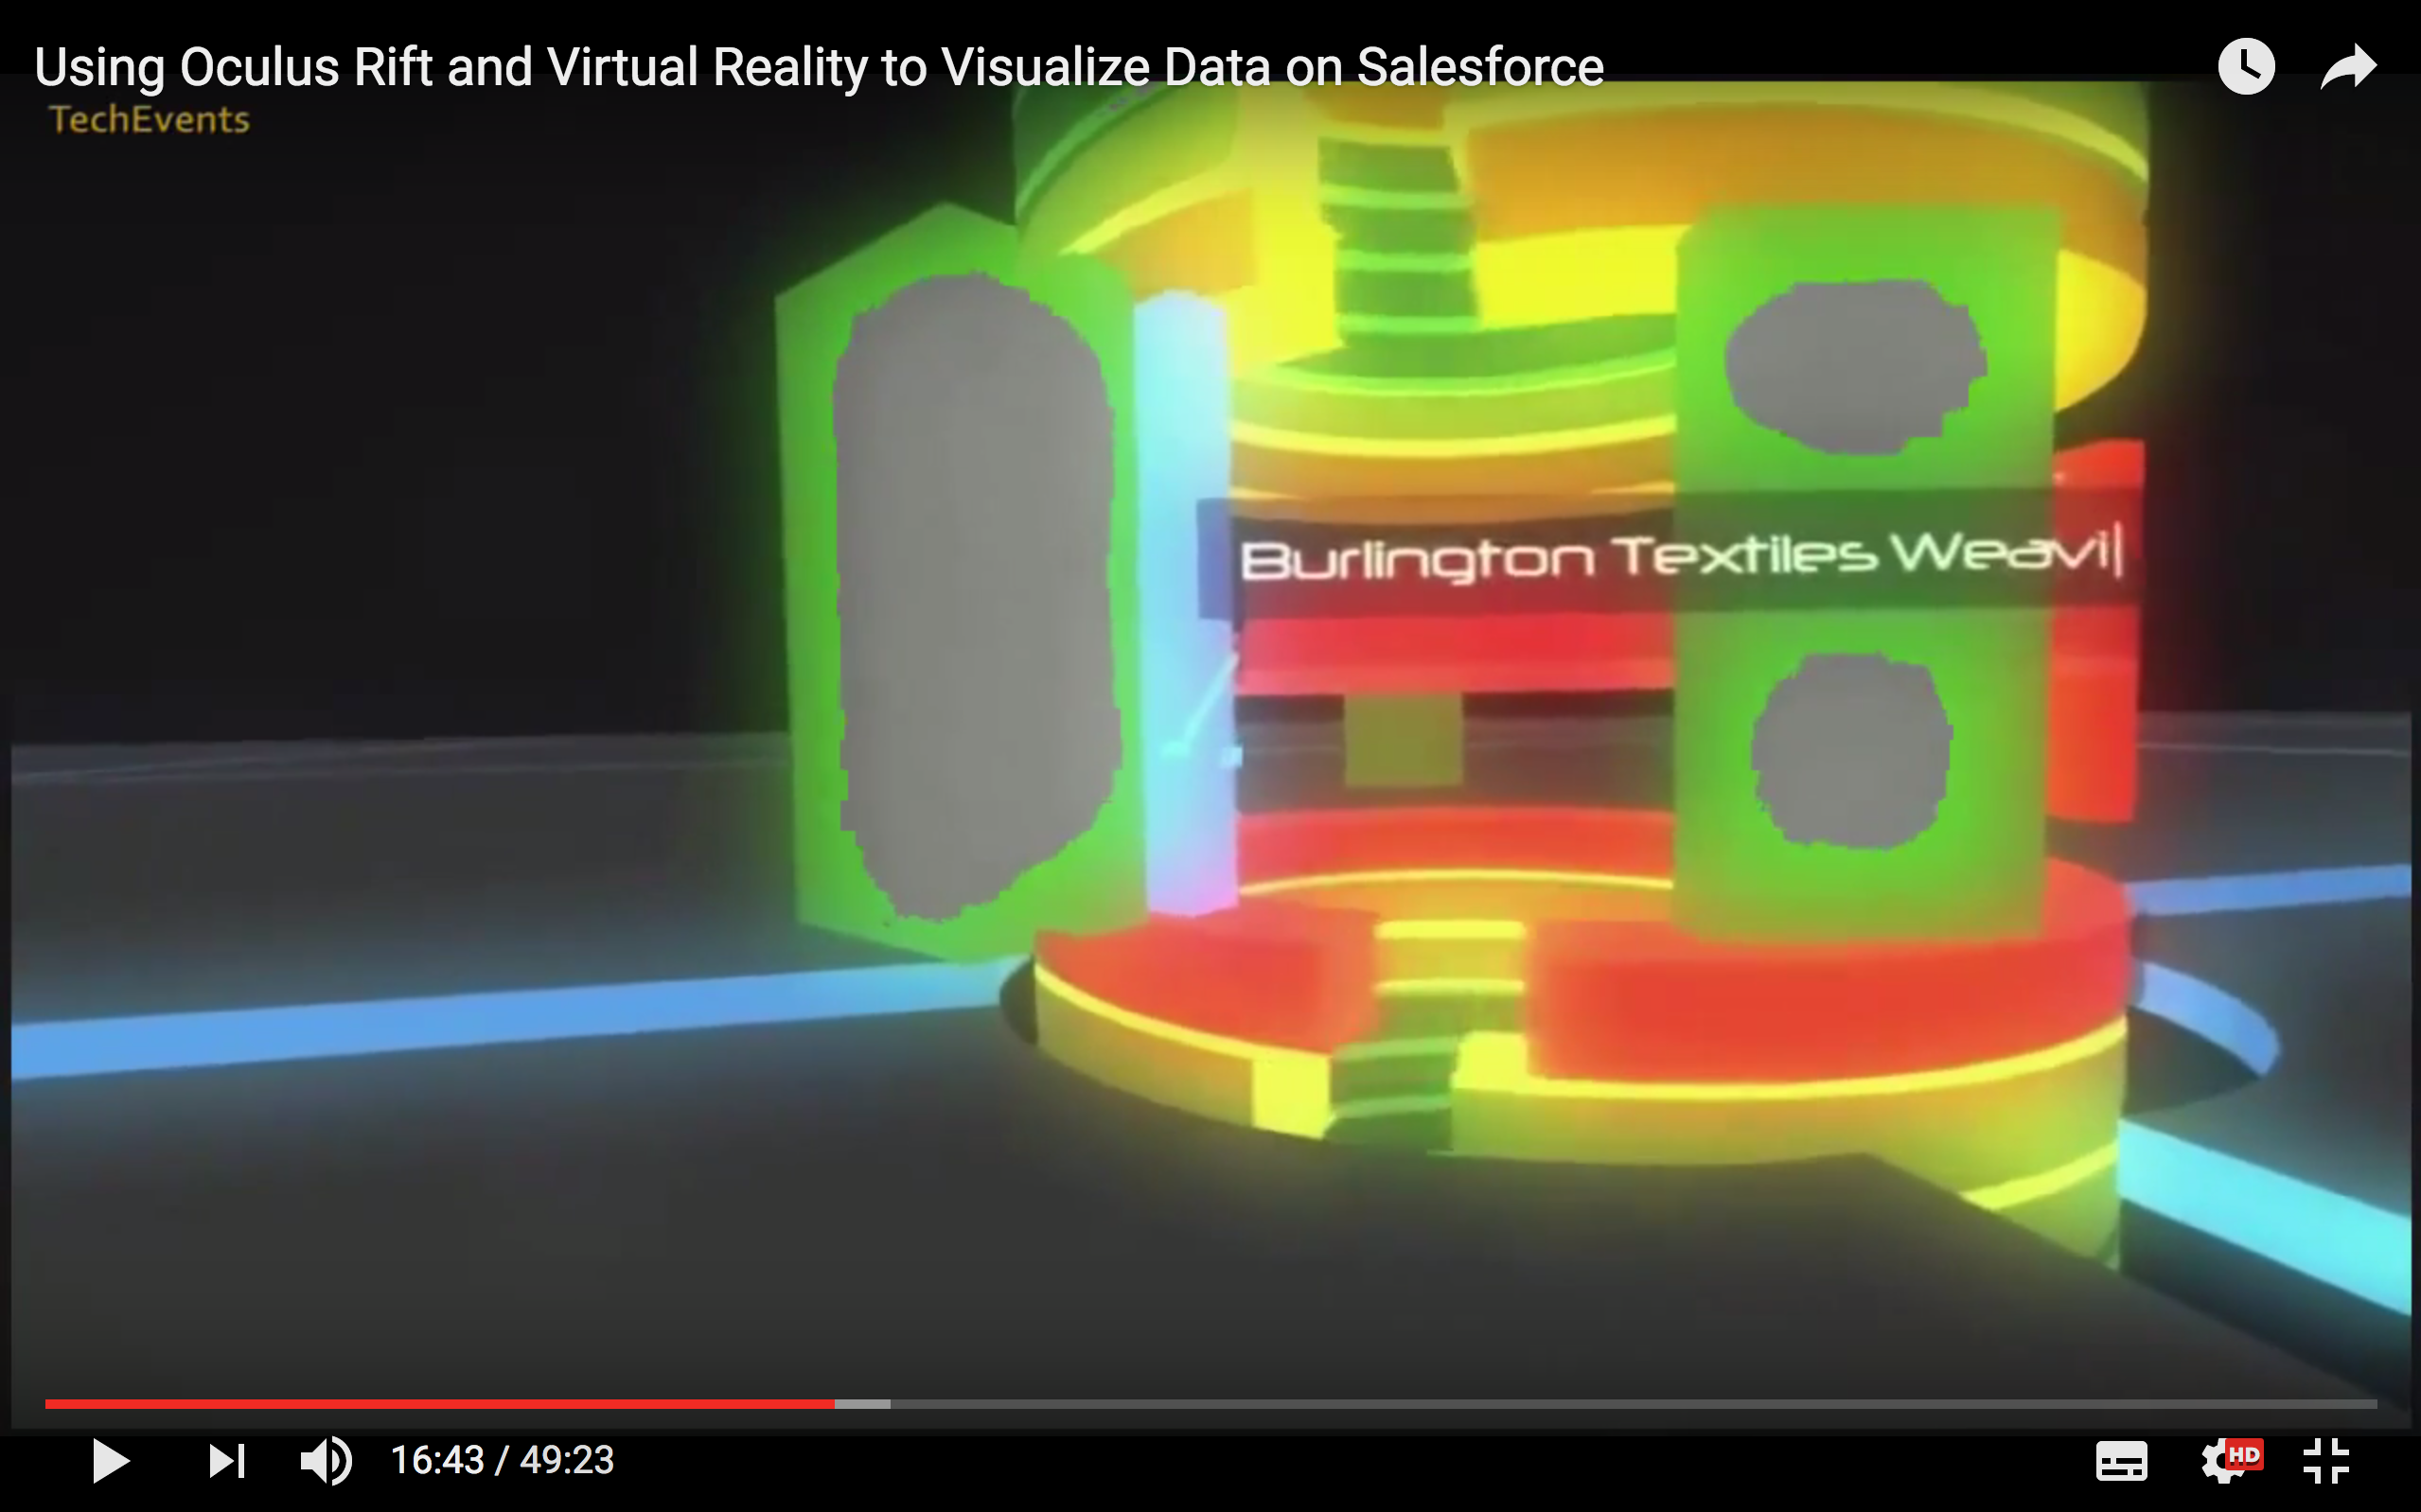
\includegraphics[width=7cm]{03_Figures/05_LitReview/CodeScience2015b.png}
		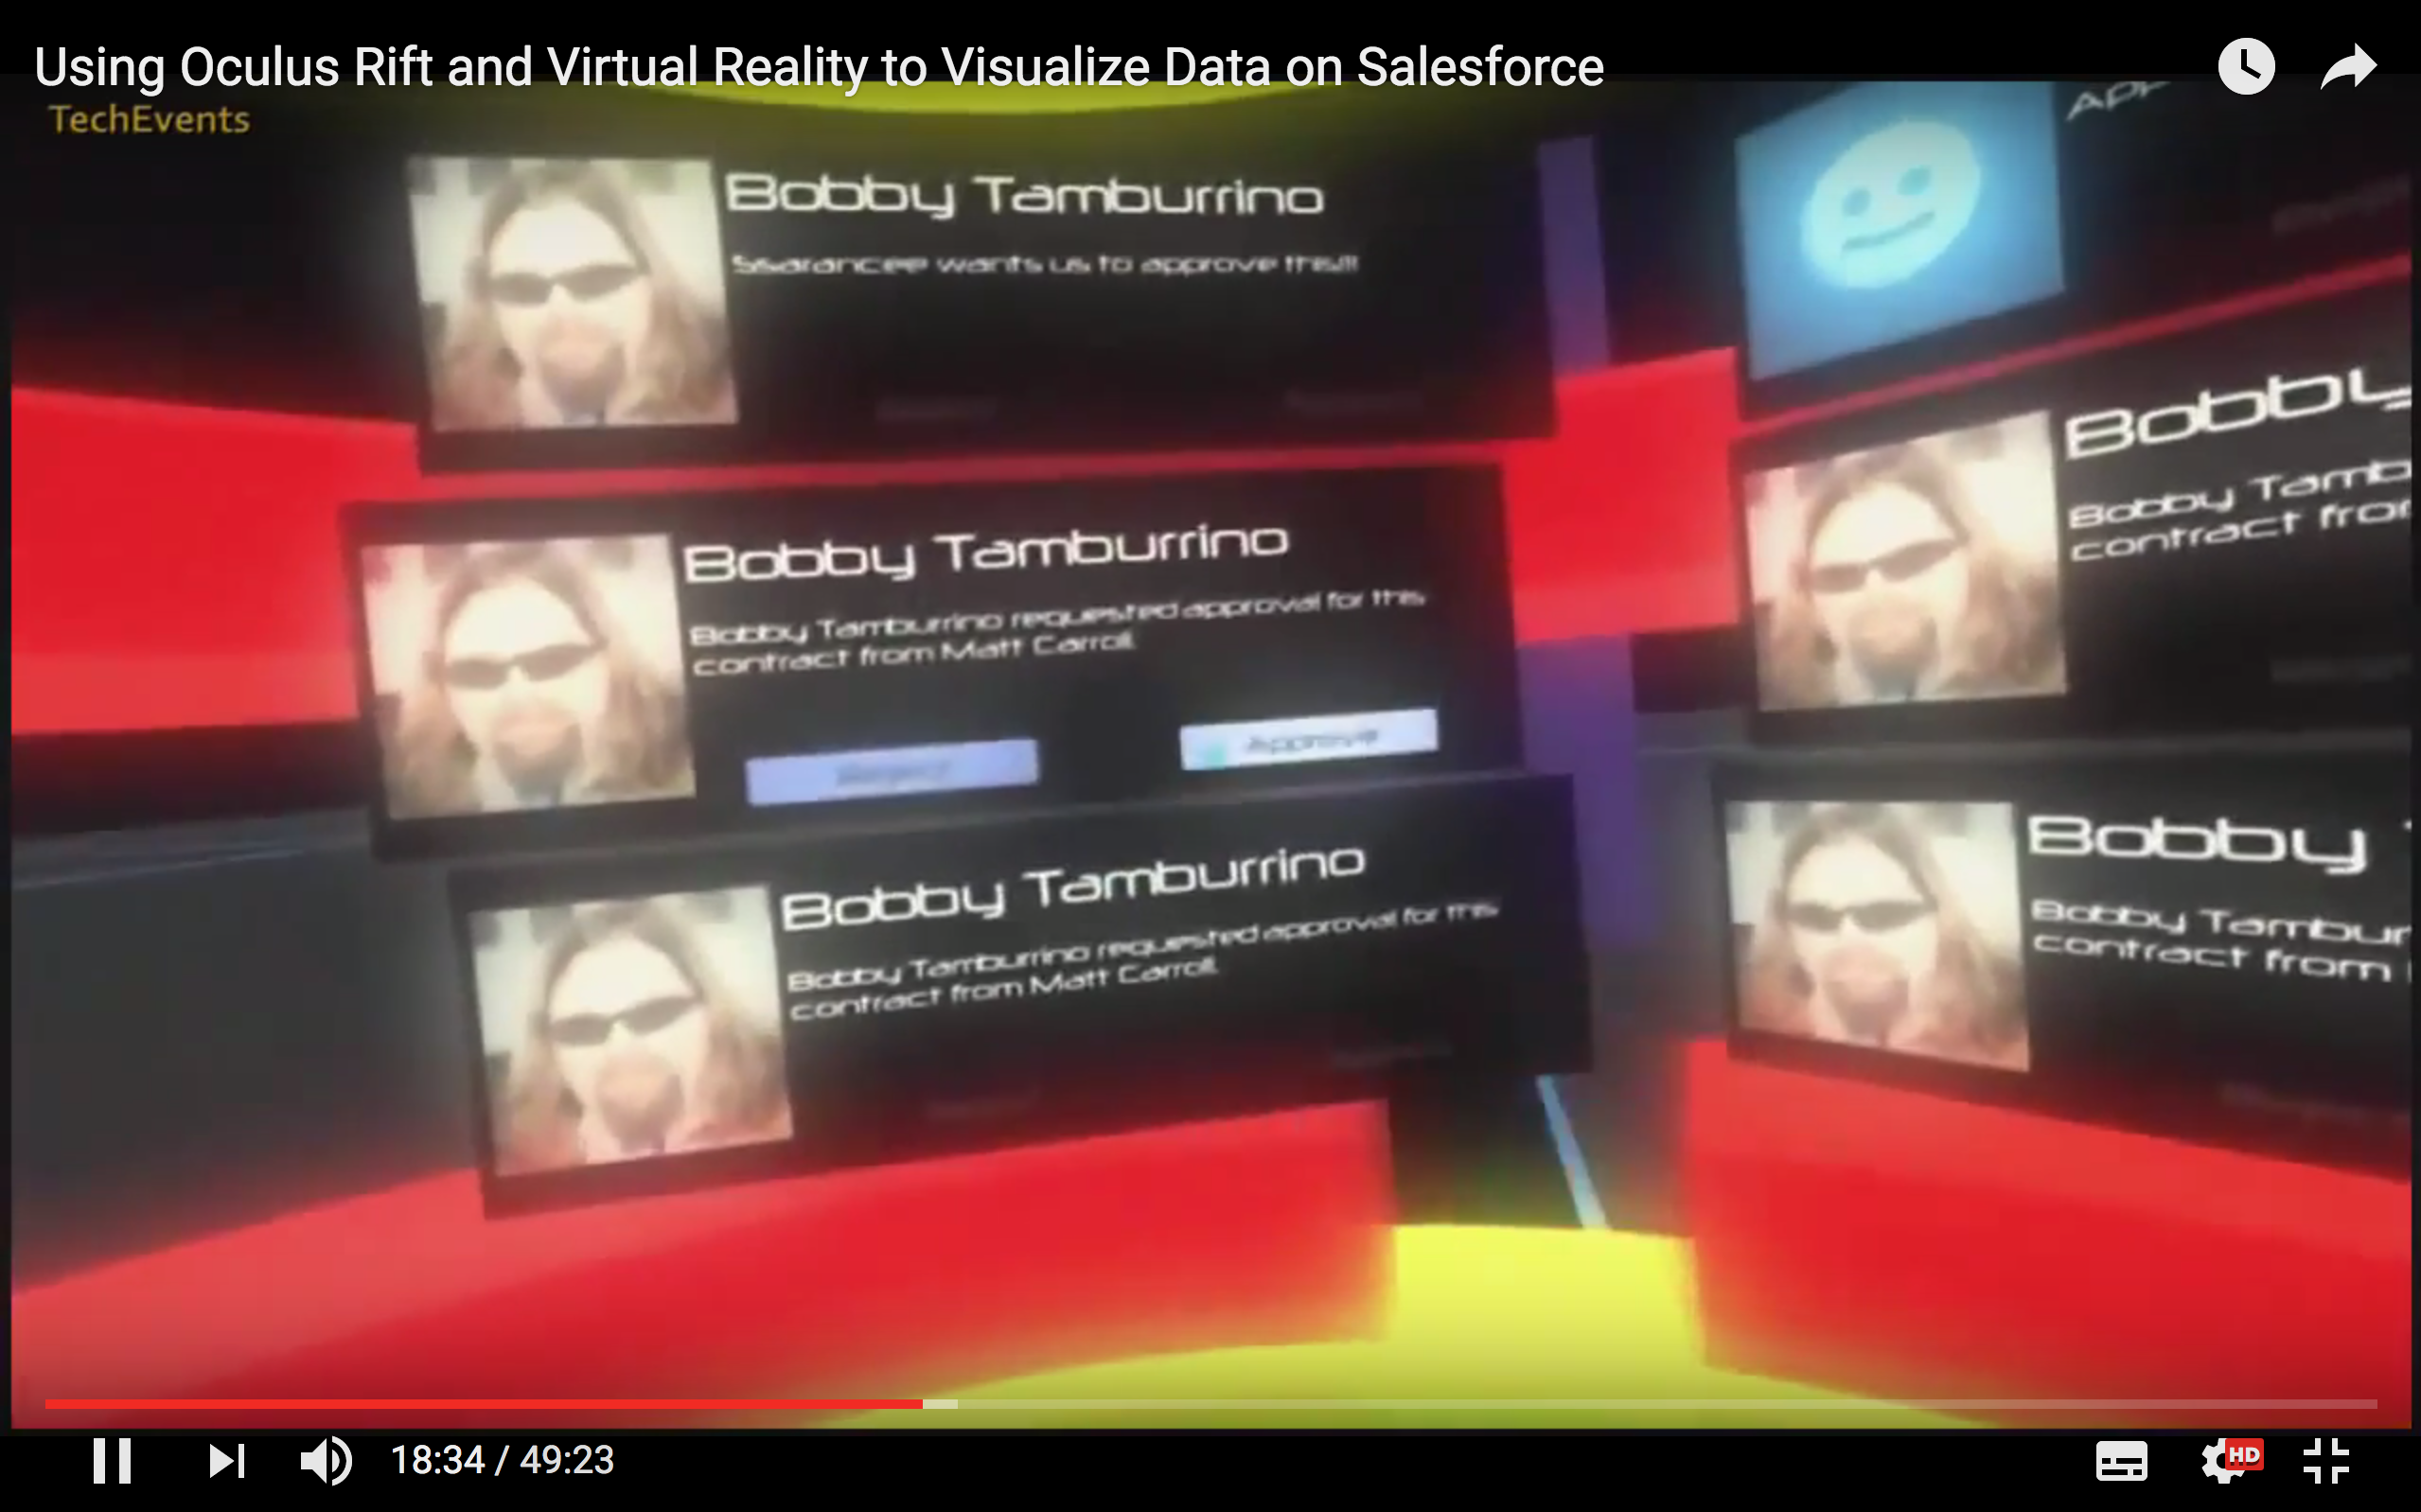
\includegraphics[width=7cm]{03_Figures/05_LitReview/CodeScience2015a.png}
		\caption[Outside view on tower built from rotating data rings with varying speed and detail view from a single ring with multiple data displays in \gls{vr}]{Outside view on tower built from rotating data rings with varying speed (1) and detail view from a single ring with multiple data displays (2) in \gls{vr} \citep{CodeScience2015}}
		\label{fig:rotatingringstoweranddetail}
	\end{center}
\end{figure}

% SOME MORE TEXT ABOUT 2D VS 3D THAT MIGHT BE USEFUL LATER
% Nevertheless, it also should be cautioned that going from 2D to 3D adds far less visual information than might be supposed. Consider the following simple argument. On a one-dimensional line of a computer display, we can perceive 1000 distinct pixels. On a 2D plane of the same display, we can display 1000 × 1000 = 1,000,000 pixels, but going to a 3D stereoscopic display only increases the number of pixels by a factor of 2, and this does not double the available information because the two images must be highly correlated for us to perceive stereoscopic depth. \cite{Ware2012}


%-----------------------------------
%	SUBSECTION 4
%-----------------------------------

\subsection{SphereViz}

\cite{Soldati2007} see the available 3D space more as a sphere around the user where information can be presented. For this, they created the 'SphereViz interface' for \gls{vr} that presents a collection of image thumbnails on this virtual sphere where the position is determined based on image properties such as total intensity, colour proportions or characterizations of the image content \citep{Soldati2007}. The visualized objects are further characterized by size, scale, and distance, which plays an important role for the goal of allowing the user to perceive the information in natural scale \citep{Soldati2007}. SphereViz heavily focuses on the benefits of spatial visualisation to build image clusters in a user friendly way and thus also provides more intuitive techniques for evaluation and searching tasks as well as for just browsing through the data.
\begin{figure}[h]
	\begin{center}
		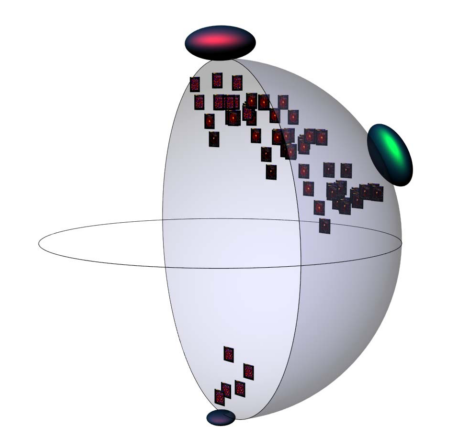
\includegraphics[width=7cm]{03_Figures/05_LitReview/Soldati2007_SphereViz.png}
		\caption[Schematic view of SphereViz where parameters influence the position of data objects]{Schematic view of SphereViz where parameters (ellipsoids) influence the position of data objects (rectangles) \citep{Soldati2007}}
		\label{fig:sphereviz}
	\end{center}
\end{figure} \newline
Figure \ref{fig:sphereviz} shows a schematic view of SphereViz where two parameters influence the position of a set of data objects. \newline
\cite{Kwon2015} also built on the idea of a virtual sphere with the benefit of having all nodes on it equally visible to the user. The relation between the nodes are indicated with edges that are however routed outside of the sphere in order to not block the view on the nodes themselves \citep{Kwon2015}. Figure \ref{fig:sphericalgraph} shows three different approaches with varying amounts of distortion that give an indication how the connections are put outside the users direct view to not interfere with the usability.
\begin{figure}[h]
	\begin{center}
		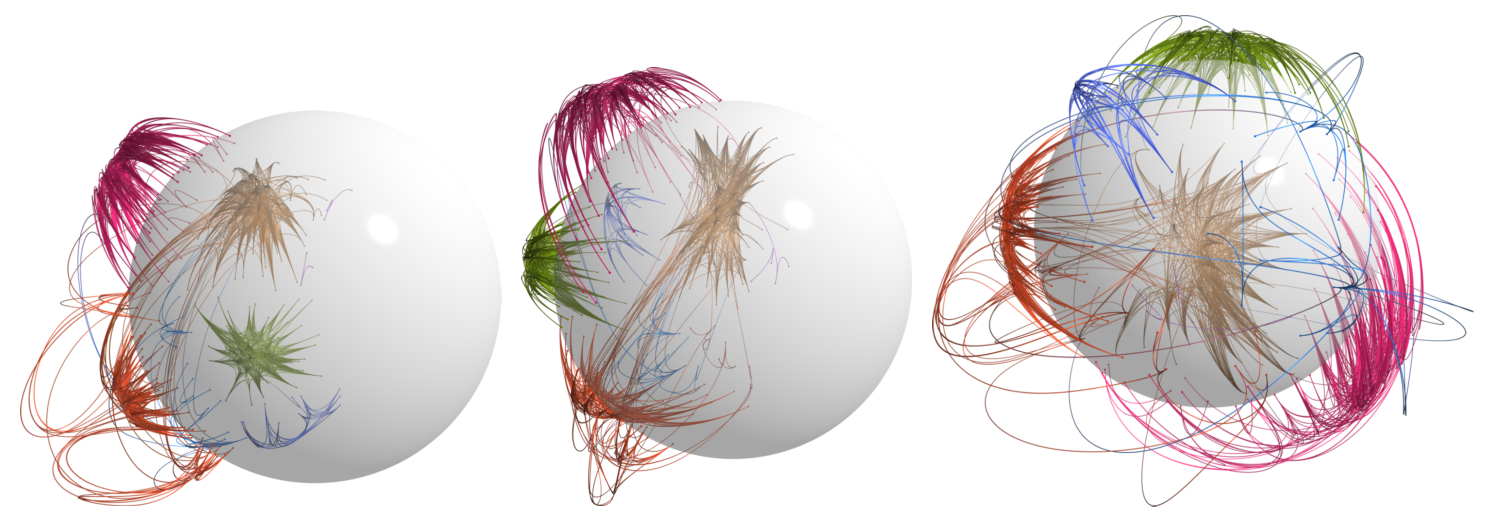
\includegraphics[width=14cm]{03_Figures/05_LitReview/Kwon2015_SphericalGraphLayout.png}
		\caption[2D layouts mapped to a sphere with varying amounts of distortion]{2D layouts mapped to a sphere with varying amounts of distortion:  \citep{Kwon2015}}
		\label{fig:sphericalgraph}
	\end{center}
\end{figure} \newline
In terms of data manipulation, \cite{Soldati2007} decided to allow the user to simply grab the parameter handles on the sphere and to move them around to see the immediate effects this has on the position of the individual data objects and thus giving valuable feedback to the user. When some data objects (i.e. thumbnails) are hidden behind others, \cite{Soldati2007} believe that it provides the best experience to let him walk around them to bring them in focus instead of bothering about more input devices. One more feature is the \gls{wim}, a small-scale representation of the whole scene that allows for a second, dynamic perspective where also direct manipulations can be done \citep{Soldati2007}. By taking the \gls{vism} into acount, \cite{Soldati2007} already covered the \textit{zoom}, \textit{filter} and \textit{details in demand} feature with \gls{wim} and planned to later extend it with the possibility for an \textit{overview} of all available data. \cite{Soldati2007} see great potential in using \gls{vr} for visually exploring multi-dimensional data sets (particularly with their SphereViz) and expect that in the next 10 to 15 years \gls{vr} will allow for completely new ways to look at and interact with large data sets.


%-----------------------------------
%	SUBSECTION 5
%-----------------------------------

\subsection{Data Forest}

As soon as there are more than three dimensions for the data, traditional visualisation patterns come at their limits and a new kind of strategy has to be applied. \cite{Stone1994} provide some examples for characteristics of virtual objects that can be applied to for allowing more dimensions:
\begin{itemize}[noitemsep,nolistsep]
	\item Size (e.g. large, medium, small)
	\item Shape (e.g. triangle, square, pentagon)
	\item Colour (e.g. red, purple, blue)
	\item Texture (photographic images can be "painted" onto objects)
	\item Position (X, Y, and Z)
	\item Orientation (roll, pitch, yaw)
	\item Behaviour (spinning, bouncing, blinking, breathing, etc.)
	\item Sound (chiming, singing, buzzing, etc.)
\end{itemize}
Upon combining them, it will become possible to also visualize data that has many more dimensions than just three in a ways that is not as abstract as introducing a fourth or fifth dimension as it is done in OLAP data cubes. \cite{Jamieson2007} applied this concept for their implementation of a 'data forest' that is made of individual data trees which represents different parameters of one data set as physical properties of the tree (i.e. trunk and crown). \cite{Jamieson2007} decided for the use of data trees since it is a simple object that people also are quite familiar with and thus can more easily make decision based on the size and shape of a tree relative to others. In specific, \cite{Jamieson2007} used the following eight parameters for the visualization:
\begin{itemize}[noitemsep,nolistsep]
	\item Position of the tree within the VE \textit{(Position)}
	\item Height of trunk \textit{(Size)}
	\item Width of trunk \textit{(Size)}
	\item Colour of trunk \textit{(Colour)}
	\item Transparency value of the trunk \textit{(Colour)}
	\item Size of crown \textit{(Size)}
	\item Colour of crown  \textit{(Colour)}
	\item Transparency value of crown  \textit{(Colour)}
\end{itemize}
By referring back to the list of characteristics from \cite{Stone1994}, the eight parameters focus on \textit{Position, Size and Colour} while the idea of the data forest itself focuses on \textit{Shape}. An example of the visualized data forest can be seen in Figure \ref{fig:dataforest}.
\begin{figure}[h]
	\begin{center}
		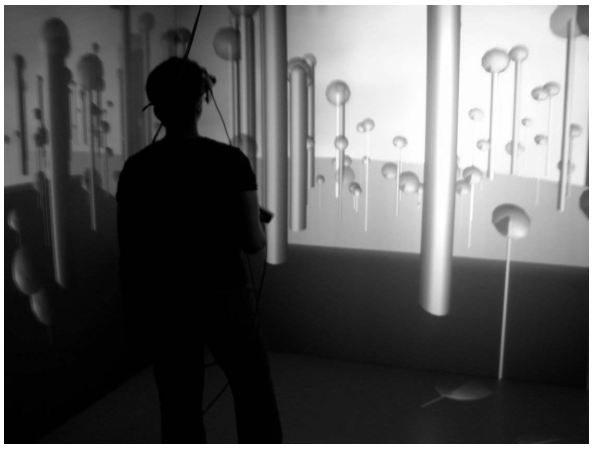
\includegraphics[width=7cm]{03_Figures/05_LitReview/Jamieson2007_DataTree.png}
		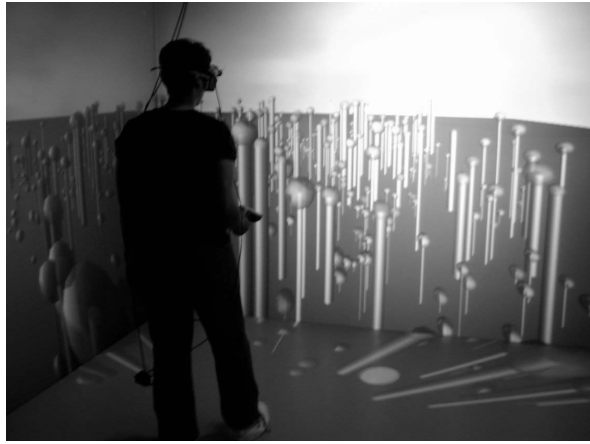
\includegraphics[width=7cm]{03_Figures/05_LitReview/Jamieson2007_DataTreeOverview.png}
		\caption[Navigation and Overview mode in a Data Forest]{Navigation (1) and Overview (2) mode in a Data Forest \citep{Jamieson2007}}
		\label{fig:dataforest}
	\end{center}
\end{figure}
The factor of time can also be applied by animating the forest and observing how the individual trees change their size and colour over time. For the implementation of the "drill down" functionality, \cite{Jamieson2007} decided to take the approach of "exposing the roots" of the data tree to get access to the underlying data. This is an elegant way as it fits together with the mood that is set with the data forest and thus also feels more natural to use. \newline
\cite{Jamieson2007} further indicate that their data forest could also be applied to stock market data where the movement of share prices can be linked to the shape and growth of the forest.


%-----------------------------------
%	SUBSECTION 6
%-----------------------------------

\subsection{Data Visualizer iViz}

A somewhat similar approach to the data forest has been research by \cite{Donalek2014} in their attempt to understand how effective data visualization can look like in the era of big data. They stated that \gls{vr} has already shown that it leads to better discovery when the primary (data) dimensions are spatial, and that the more dimensions can be visualized effectively, the higher the chances are to recognize potentially interesting patterns \citep{Donalek2014}. Their initial attempts were with the OpenSim based virtual world called 'vCalltech' that allowed \cite{Donalek2014} to easily visualize around $10^{4}$ - $10^{5}$ data objects. Figure \ref{fig:caltechsim} shows such a visualization with 'vCallTech' where different parameter values are mapped to the XYZ axis, the data point shapes, sizes, colours and also transparencies, allowing for a representation of an 8-dimensional data visualisation \citep{Donalek2014}.
\begin{figure}[h]
	\begin{center}
		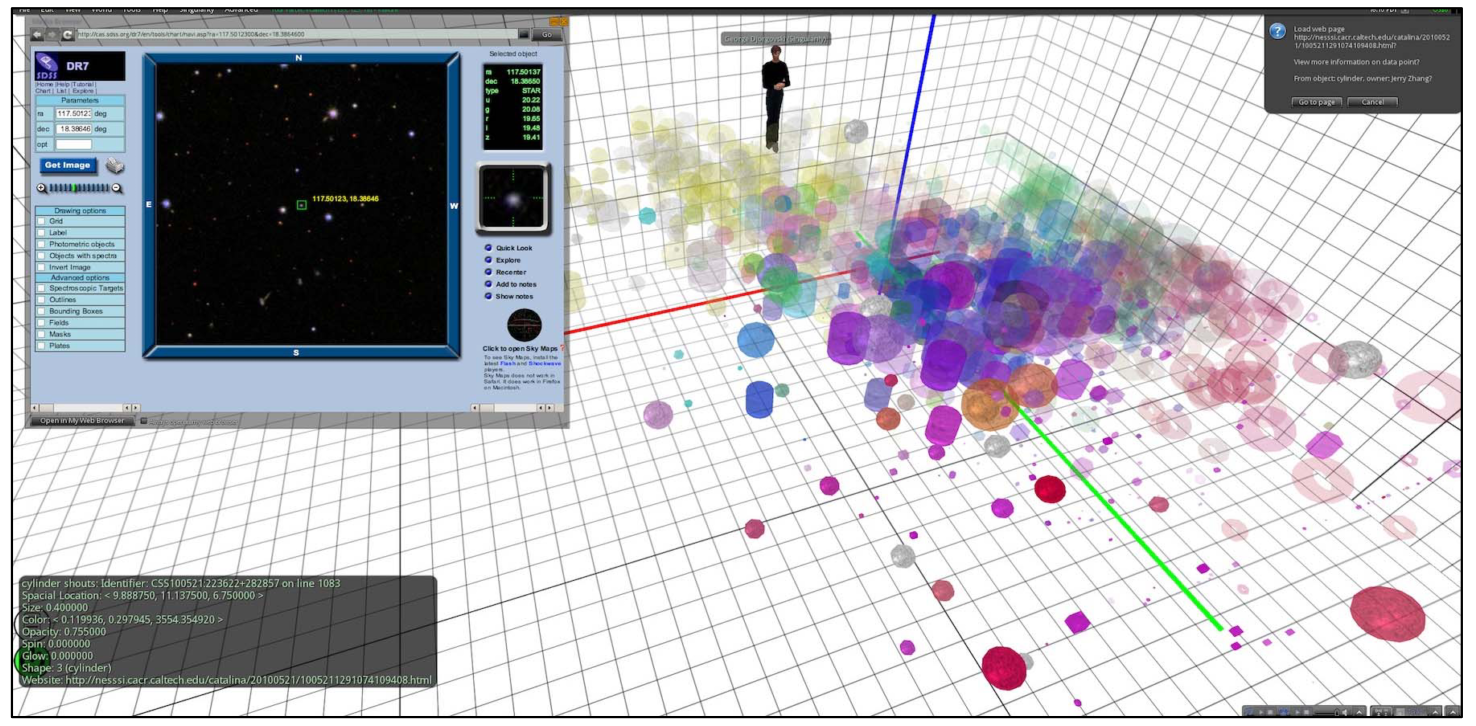
\includegraphics[width=14cm]{03_Figures/05_LitReview/Donalek2014_Caltech.png}
		\caption[Data visualization experiments in the OpenSim-based virtual world vCaltech]{Data visualization experiments in the OpenSim-based virtual world vCaltech \citep{Donalek2014}}
		\label{fig:caltechsim}
	\end{center}
\end{figure}

Soon, \cite{Donalek2014} realised that while \gls{ots} products have multiple advantages, they often are not fully optimised for an efficient rendering of big data sets and only provide limited functionalities for customized scripting. With their own Unity-based implementation called 'iViz', \cite{Donalek2014} also added a new collaborative feature which allows for a multi-user visual data exploration where each user not only has his own viewpoint but can also broadcast his view to a shared view accessible to all users. \cite{Donalek2014} also further improved the performance to be able to rapidly visualize more than $10^{5}$ - $10^{6}$ data points, as also shown in Figure \ref{fig:iviz}. Their user interface for 'iViz' allows to easily change the mapping of individual data parameters to the graphical dimensions (i.e. XYZ position, colour, shape, size, ...) which should improve the data exploration as clusters and outliers might become more obvious based on the chosen mapping \citep{Donalek2014}. Although this allows for a very flexible and powerful way to visually explore data and discover new patterns, there is no direct interaction with the data possible.
\begin{figure}[h]
	\begin{center}
		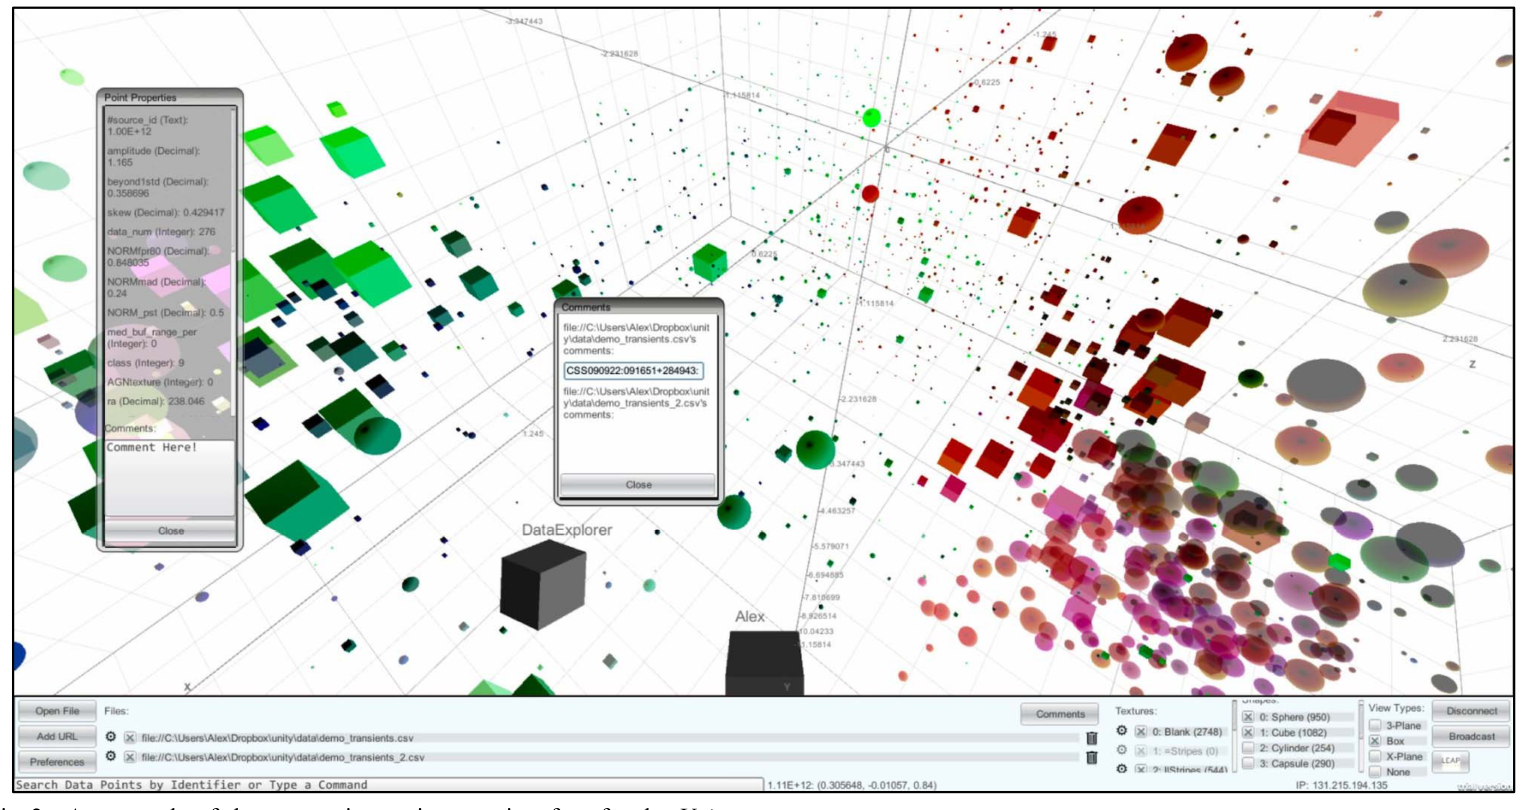
\includegraphics[width=14cm]{03_Figures/05_LitReview/Donalek2014_iViz.png}
		\caption[Example of an interactive user interface for the Unity-based data visualizer, iViz]{Example of an interactive user interface for the Unity-based data visualizer, iViz \citep{Donalek2014}}
		\label{fig:iviz}
	\end{center}
\end{figure}

%-----------------------------------
%	SUBSECTION 7
%-----------------------------------

\subsection{Other Applications}

Another similar approach to the Data Forest and iViz, although not in \gls{vr}, has been applied to the city building simulation PC Game "Cities: Skylines", published by \cite{Paradox2014}, where certain info views such as the fire safety has been directly visually applied to the city. Figure \ref{fig:citiesskylinesfiresafety} shows how this looks like when the houses are coloured depending on their relative fire safety. This presentation technique could also be applied in \gls{vr} without many changes, especially since \cite{Google2016a} has released a \gls{vr}-ready version of Google Earth in November 2016.
\begin{figure}[b]
	\begin{center}
		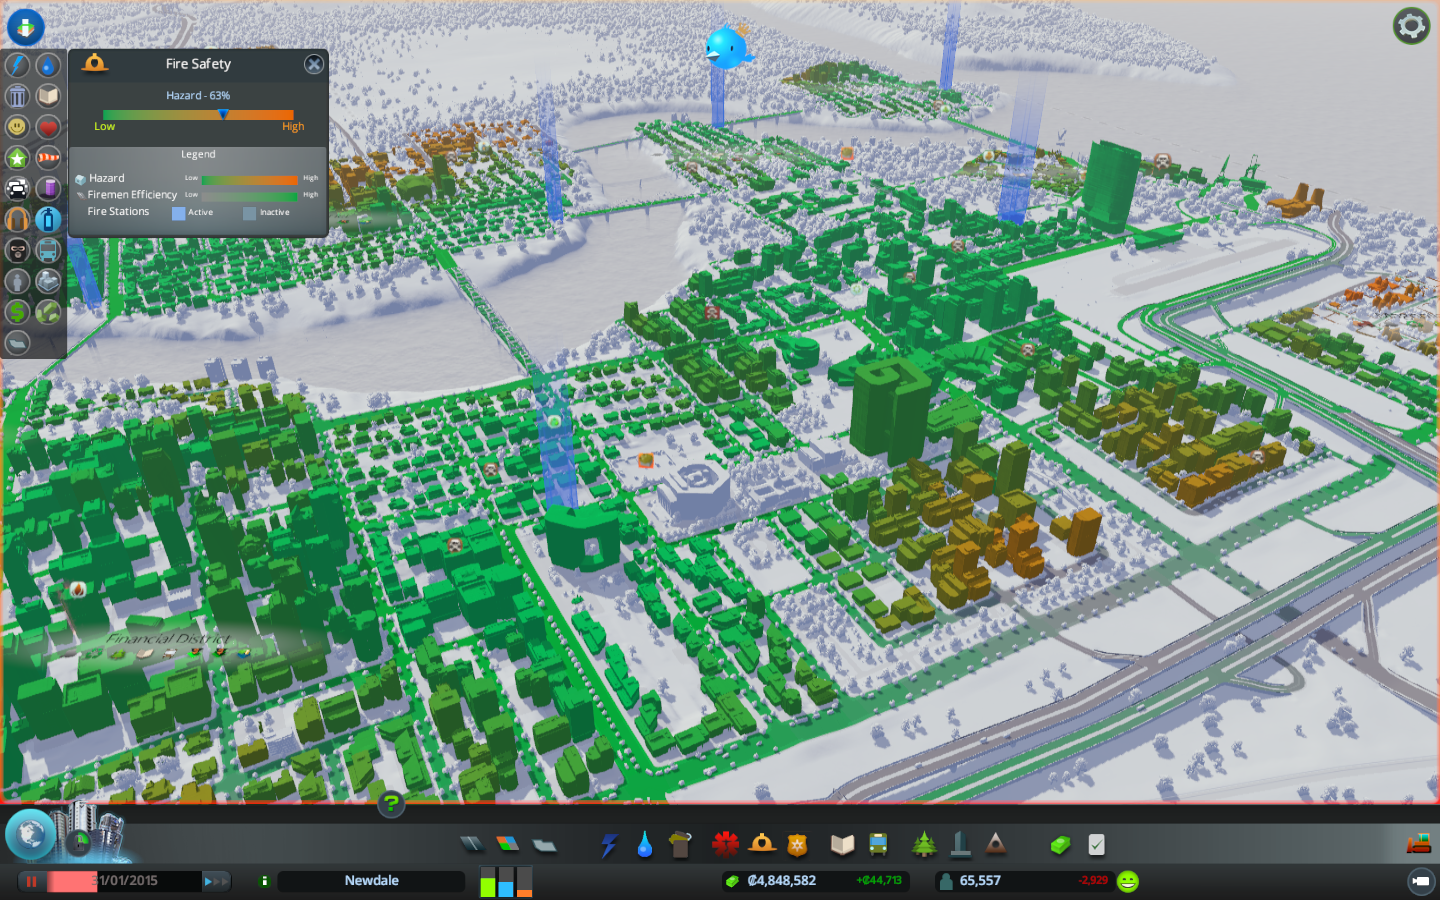
\includegraphics[width=10cm]{03_Figures/05_LitReview/ParadoxWiki2014_CitiesSkylines.png}
		\caption[Fire Safety Info View in Cities: Skylines]{Fire Safety Info View in Cities: Skylines \citep{Paradox2014}}
		\label{fig:citiesskylinesfiresafety}
	\end{center}
\end{figure}


%-----------------------------------
%	SUBSECTION 4
%-----------------------------------

\subsection{Conclusion}

It can be seen, that it very much depends on the type of data that shall be visualized and the amount of parameters a single data object has in order to find a good model and technique that brings the most benefit to the users. While the sphere is a more generic approach that can be ideal for clustering data based on a smaller amount of influencing parameters, the iViz implementation shows a a more large-scale approach which however relies on more abstract objects. The presentation with more familiar 3D objects such as in the data forest is much more natural to us and thus also easier to understand and interact with for inexperienced users. \newline
The chosen presentation also has an influence on what kind of interactions can be offered to the user and how the data exploration can be conducted in the most effective way. While some models primarily focus on pattern-finding without direct interaction on a single data object, other models provide rich user experience with very detailed actions to not only view, but also work with the data. One thing that many models have in common is the use of changing size and colour of certain objects to visual certain states of them, compared to the other data objects. Furthermore, it also has been shown that traditional 2D charts can be successfully applied to \gls{vr} environment without many changes and still provide benefits compared to the 2D-display counterparts. \newline
In terms of interacting with the visualisations, it is interesting to see that none of the before discussed applications actually implemented any "zoom" in the way it is known from 2D applications, but rather allow the user to freely navigate around in the \gls{ve} and get as close to the data as desired. Also context-menus barely seen any use, where it can be assumed that they are only rarely used since they can be seen as something "unnatural" that does exist in our real world.


%----------------------------------------------------------------------------------------
%	SECTION 4
%----------------------------------------------------------------------------------------

\section{Conclusion}

\label{SectionLiteratureReviewConclusion}

A broad range of different methods for user input, interaction patterns and also models for how data can be visualized and interacted with exist. There is no unique single combination that is the best, since it always depends on what kind of data is available and what the goal of the visualisation in \gls{vr} should be. One important factor about the success of a \gls{vr} application showed itself throughout the whole literature review: Immersion. From how our intended actions are brought into \gls{vr}, over the interaction patterns with the data, to the visualisation with practical examples itself; it is crucial that the user feels immersed and can intuitively navigate around in the \gls{ve}. \newline
In the next chapter, the research methodology of this thesis is described.
